% Options for packages loaded elsewhere
\PassOptionsToPackage{unicode}{hyperref}
\PassOptionsToPackage{hyphens}{url}
%
\documentclass[
]{book}
\usepackage{amsmath,amssymb}
\usepackage{iftex}
\ifPDFTeX
  \usepackage[T1]{fontenc}
  \usepackage[utf8]{inputenc}
  \usepackage{textcomp} % provide euro and other symbols
\else % if luatex or xetex
  \usepackage{unicode-math} % this also loads fontspec
  \defaultfontfeatures{Scale=MatchLowercase}
  \defaultfontfeatures[\rmfamily]{Ligatures=TeX,Scale=1}
\fi
\usepackage{lmodern}
\ifPDFTeX\else
  % xetex/luatex font selection
\fi
% Use upquote if available, for straight quotes in verbatim environments
\IfFileExists{upquote.sty}{\usepackage{upquote}}{}
\IfFileExists{microtype.sty}{% use microtype if available
  \usepackage[]{microtype}
  \UseMicrotypeSet[protrusion]{basicmath} % disable protrusion for tt fonts
}{}
\makeatletter
\@ifundefined{KOMAClassName}{% if non-KOMA class
  \IfFileExists{parskip.sty}{%
    \usepackage{parskip}
  }{% else
    \setlength{\parindent}{0pt}
    \setlength{\parskip}{6pt plus 2pt minus 1pt}}
}{% if KOMA class
  \KOMAoptions{parskip=half}}
\makeatother
\usepackage{xcolor}
\usepackage{color}
\usepackage{fancyvrb}
\newcommand{\VerbBar}{|}
\newcommand{\VERB}{\Verb[commandchars=\\\{\}]}
\DefineVerbatimEnvironment{Highlighting}{Verbatim}{commandchars=\\\{\}}
% Add ',fontsize=\small' for more characters per line
\usepackage{framed}
\definecolor{shadecolor}{RGB}{248,248,248}
\newenvironment{Shaded}{\begin{snugshade}}{\end{snugshade}}
\newcommand{\AlertTok}[1]{\textcolor[rgb]{0.94,0.16,0.16}{#1}}
\newcommand{\AnnotationTok}[1]{\textcolor[rgb]{0.56,0.35,0.01}{\textbf{\textit{#1}}}}
\newcommand{\AttributeTok}[1]{\textcolor[rgb]{0.13,0.29,0.53}{#1}}
\newcommand{\BaseNTok}[1]{\textcolor[rgb]{0.00,0.00,0.81}{#1}}
\newcommand{\BuiltInTok}[1]{#1}
\newcommand{\CharTok}[1]{\textcolor[rgb]{0.31,0.60,0.02}{#1}}
\newcommand{\CommentTok}[1]{\textcolor[rgb]{0.56,0.35,0.01}{\textit{#1}}}
\newcommand{\CommentVarTok}[1]{\textcolor[rgb]{0.56,0.35,0.01}{\textbf{\textit{#1}}}}
\newcommand{\ConstantTok}[1]{\textcolor[rgb]{0.56,0.35,0.01}{#1}}
\newcommand{\ControlFlowTok}[1]{\textcolor[rgb]{0.13,0.29,0.53}{\textbf{#1}}}
\newcommand{\DataTypeTok}[1]{\textcolor[rgb]{0.13,0.29,0.53}{#1}}
\newcommand{\DecValTok}[1]{\textcolor[rgb]{0.00,0.00,0.81}{#1}}
\newcommand{\DocumentationTok}[1]{\textcolor[rgb]{0.56,0.35,0.01}{\textbf{\textit{#1}}}}
\newcommand{\ErrorTok}[1]{\textcolor[rgb]{0.64,0.00,0.00}{\textbf{#1}}}
\newcommand{\ExtensionTok}[1]{#1}
\newcommand{\FloatTok}[1]{\textcolor[rgb]{0.00,0.00,0.81}{#1}}
\newcommand{\FunctionTok}[1]{\textcolor[rgb]{0.13,0.29,0.53}{\textbf{#1}}}
\newcommand{\ImportTok}[1]{#1}
\newcommand{\InformationTok}[1]{\textcolor[rgb]{0.56,0.35,0.01}{\textbf{\textit{#1}}}}
\newcommand{\KeywordTok}[1]{\textcolor[rgb]{0.13,0.29,0.53}{\textbf{#1}}}
\newcommand{\NormalTok}[1]{#1}
\newcommand{\OperatorTok}[1]{\textcolor[rgb]{0.81,0.36,0.00}{\textbf{#1}}}
\newcommand{\OtherTok}[1]{\textcolor[rgb]{0.56,0.35,0.01}{#1}}
\newcommand{\PreprocessorTok}[1]{\textcolor[rgb]{0.56,0.35,0.01}{\textit{#1}}}
\newcommand{\RegionMarkerTok}[1]{#1}
\newcommand{\SpecialCharTok}[1]{\textcolor[rgb]{0.81,0.36,0.00}{\textbf{#1}}}
\newcommand{\SpecialStringTok}[1]{\textcolor[rgb]{0.31,0.60,0.02}{#1}}
\newcommand{\StringTok}[1]{\textcolor[rgb]{0.31,0.60,0.02}{#1}}
\newcommand{\VariableTok}[1]{\textcolor[rgb]{0.00,0.00,0.00}{#1}}
\newcommand{\VerbatimStringTok}[1]{\textcolor[rgb]{0.31,0.60,0.02}{#1}}
\newcommand{\WarningTok}[1]{\textcolor[rgb]{0.56,0.35,0.01}{\textbf{\textit{#1}}}}
\usepackage{longtable,booktabs,array}
\usepackage{calc} % for calculating minipage widths
% Correct order of tables after \paragraph or \subparagraph
\usepackage{etoolbox}
\makeatletter
\patchcmd\longtable{\par}{\if@noskipsec\mbox{}\fi\par}{}{}
\makeatother
% Allow footnotes in longtable head/foot
\IfFileExists{footnotehyper.sty}{\usepackage{footnotehyper}}{\usepackage{footnote}}
\makesavenoteenv{longtable}
\usepackage{graphicx}
\makeatletter
\newsavebox\pandoc@box
\newcommand*\pandocbounded[1]{% scales image to fit in text height/width
  \sbox\pandoc@box{#1}%
  \Gscale@div\@tempa{\textheight}{\dimexpr\ht\pandoc@box+\dp\pandoc@box\relax}%
  \Gscale@div\@tempb{\linewidth}{\wd\pandoc@box}%
  \ifdim\@tempb\p@<\@tempa\p@\let\@tempa\@tempb\fi% select the smaller of both
  \ifdim\@tempa\p@<\p@\scalebox{\@tempa}{\usebox\pandoc@box}%
  \else\usebox{\pandoc@box}%
  \fi%
}
% Set default figure placement to htbp
\def\fps@figure{htbp}
\makeatother
\setlength{\emergencystretch}{3em} % prevent overfull lines
\providecommand{\tightlist}{%
  \setlength{\itemsep}{0pt}\setlength{\parskip}{0pt}}
\setcounter{secnumdepth}{5}
\usepackage{booktabs}
\usepackage[]{natbib}
\bibliographystyle{apalike}
\usepackage{bookmark}
\IfFileExists{xurl.sty}{\usepackage{xurl}}{} % add URL line breaks if available
\urlstyle{same}
\hypersetup{
  pdftitle={Manual de uso de Makurhini},
  pdfauthor={Oscar Godínez Gómez},
  hidelinks,
  pdfcreator={LaTeX via pandoc}}

\title{Manual de uso de Makurhini}
\author{Oscar Godínez Gómez}
\date{2025-07-16}

\begin{document}
\maketitle

{
\setcounter{tocdepth}{1}
\tableofcontents
}
\chapter*{Makurhini}\label{makurhini}
\addcontentsline{toc}{chapter}{Makurhini}


\includegraphics[width=2.08333in,height=\textheight,keepaspectratio]{LOGO_MAKHURINI.png}

En este manual se documenta parte de las funciones del paquete Makurhini

\chapter{Instalación del paquete Makurhini}\label{instalaciuxf3n-del-paquete-makurhini}

\section{Instalación estandar}\label{instalaciuxf3n-estandar}

\begin{itemize}
\tightlist
\item
  Depende de R (\textgreater{} 4.0.0), igraph (\textgreater= 1.2.6)
\end{itemize}

\begin{Shaded}
\begin{Highlighting}[]
\FunctionTok{install.packages}\NormalTok{(}\StringTok{"igraph"}\NormalTok{)}
\end{Highlighting}
\end{Shaded}

\begin{itemize}
\item
  Se recomienda pre-instalar Rtools:
  \url{https://cran.r-project.org/bin/windows/Rtools/}
\item
  Se recomienda pre-instalar los paquetes devtools y remotes
\end{itemize}

\begin{Shaded}
\begin{Highlighting}[]
\FunctionTok{install.packages}\NormalTok{(}\FunctionTok{c}\NormalTok{(}\StringTok{"devtools"}\NormalTok{, }\StringTok{"remotes"}\NormalTok{))}
\end{Highlighting}
\end{Shaded}

\begin{Shaded}
\begin{Highlighting}[]
\FunctionTok{library}\NormalTok{(devtools) }
\FunctionTok{library}\NormalTok{(remotes)}
\FunctionTok{install\_github}\NormalTok{(}\StringTok{"connectscape/Makurhini"}\NormalTok{, }\AttributeTok{dependencies =} \ConstantTok{TRUE}\NormalTok{, }\AttributeTok{upgrade =} \StringTok{"never"}\NormalTok{)}
\end{Highlighting}
\end{Shaded}

En caso de que no aparezca en la lista de paquetes, cierre la sesión de
R y vuelva a abrirla.

\textbf{Si se produce el siguiente error durante la instalación:}

\begin{Shaded}
\begin{Highlighting}[]
\NormalTok{Using github PAT}
\NormalTok{from envvar GITHUB\_PAT Error}\SpecialCharTok{:}\NormalTok{ Failed to install }\StringTok{\textquotesingle{}unknown package\textquotesingle{}}\NormalTok{ from}
\NormalTok{GitHub}\SpecialCharTok{:}\NormalTok{ HTTP error }\FloatTok{401.}\NormalTok{ Bad credentials}
\end{Highlighting}
\end{Shaded}

\textbf{Entonces intenta lo siguiente:}

\begin{Shaded}
\begin{Highlighting}[]
\FunctionTok{Sys.getenv}\NormalTok{(}\StringTok{"GITHUB\_PAT"}\NormalTok{) }
\FunctionTok{Sys.unsetenv}\NormalTok{(}\StringTok{"GITHUB\_PAT"}\NormalTok{)}
\end{Highlighting}
\end{Shaded}

\section{Instalar en Linux}\label{instalar-en-linux}

Makurhini en Linux Para instalar Makurhini en linux considere los
siguientes pasos:

Utilice la línea de comandos de Linux para instalar el paquete de la
unidad:

\begin{Shaded}
\begin{Highlighting}[]
\NormalTok{sudo apt}\SpecialCharTok{{-}}\NormalTok{get install }\SpecialCharTok{{-}}\NormalTok{y libudunits2}\SpecialCharTok{{-}}\NormalTok{dev}
\end{Highlighting}
\end{Shaded}

Utilice la línea de comandos de Linux para instalar gdal:

\begin{Shaded}
\begin{Highlighting}[]
\NormalTok{sudo apt install libgdal}\SpecialCharTok{{-}}\NormalTok{dev}
\end{Highlighting}
\end{Shaded}

Utilice la línea de comandos de Linux para instalar libfontconfig y
libharfbuzz:

\begin{Shaded}
\begin{Highlighting}[]
\NormalTok{sudo apt install libfontconfig1}\SpecialCharTok{{-}}\NormalTok{dev}

\NormalTok{sudo apt install libharfbuzz}\SpecialCharTok{{-}}\NormalTok{dev libfribidi}\SpecialCharTok{{-}}\NormalTok{dev}
\end{Highlighting}
\end{Shaded}

Ahora puede instalar los paquetes devtools y remotes, y los paquetes
terra, raster y sf directamente en su R o RStudio.

\begin{Shaded}
\begin{Highlighting}[]
\FunctionTok{install.packages}\NormalTok{(}\FunctionTok{c}\NormalTok{(}\StringTok{\textquotesingle{}remotes\textquotesingle{}}\NormalTok{, }\StringTok{\textquotesingle{}devtools\textquotesingle{}}\NormalTok{, }\StringTok{\textquotesingle{}terra\textquotesingle{}}\NormalTok{, }\StringTok{\textquotesingle{}raster\textquotesingle{}}\NormalTok{, }\StringTok{\textquotesingle{}sf\textquotesingle{}}\NormalTok{))}
\end{Highlighting}
\end{Shaded}

Utiliza la línea de comandos de Linux para instalar igraph:

\begin{Shaded}
\begin{Highlighting}[]
\NormalTok{sudo apt}\SpecialCharTok{{-}}\NormalTok{get install libnlopt}\SpecialCharTok{{-}}\NormalTok{dev}

\NormalTok{sudo apt}\SpecialCharTok{{-}}\NormalTok{get install r}\SpecialCharTok{{-}}\NormalTok{cran}\SpecialCharTok{{-}}\NormalTok{igraph}
\end{Highlighting}
\end{Shaded}

Ahora puede instalar los paquetes gdistance, graph4lg y ggpubr
directamente en su R o RStudio.

\begin{Shaded}
\begin{Highlighting}[]
\FunctionTok{install.packages}\NormalTok{(}\FunctionTok{c}\NormalTok{(}\StringTok{\textquotesingle{}gdistance\textquotesingle{}}\NormalTok{, }\StringTok{\textquotesingle{}graph4lg\textquotesingle{}}\NormalTok{, }\StringTok{\textquotesingle{}ggpubr\textquotesingle{}}\NormalTok{))}
\end{Highlighting}
\end{Shaded}

Ahora puedes instalar Makurhini directamente en tu R o RStudio.

\begin{Shaded}
\begin{Highlighting}[]
\FunctionTok{library}\NormalTok{(devtools) }
\FunctionTok{library}\NormalTok{(remotes) }
\FunctionTok{install\_github}\NormalTok{(}\StringTok{"connectscape/Makurhini"}\NormalTok{, }\AttributeTok{dependencies =} \ConstantTok{TRUE}\NormalTok{, }\AttributeTok{upgrade =} \StringTok{"never"}\NormalTok{) }
\end{Highlighting}
\end{Shaded}

Tenga en cuenta que la instalación de Makurhini en Linux depende de su
versión del sistema operativo y de que consiga instalar los paquetes de
los que depende Makurhini.

\chapter{Estadísticas de fragmentación del paisaje}\label{estaduxedsticas-de-fragmentaciuxf3n-del-paisaje}

Exploraremos la función \textbf{\texttt{MK\_Fragmentation()}} para caracterizar la composición y la configuración espacial de los parches en nuestro paisaje.

La función calcula \textbf{ocho métricas a nivel de nodo} (como el área de nodo, el porcentaje de borde y la dimensión fractal) y \textbf{13 estadísticas de fragmentación a nivel de paisaje} (como el número de nodos, el tamaño medio, la densidad de borde y el tamaño efectivo de la malla).

Las entradas incluyen un \textbf{objeto vectorial} que representa los nodos del paisaje y un parámetro que define la distancia o profundidad de la influencia del borde (es decir, la distancia al borde del nodo).

Los resultados consisten en un \textbf{archivo vectorial tipo poligonal} que contiene métricas a nivel de nodo y \textbf{una tabla} que detalla las métricas a nivel de paisaje.

\section{Inputs}\label{inputs}

Usaremos la librerias sf, para trabajar con un shapefile que contiene 404 parches de vegetación con la menor alteración o signos de degradación en un estado de México llamado Michoacán. Tambien cargaremos el paisaje de estudio donde se encuentran los parches y que fue delimitado usando el limite politico del estado y la región fisiográfica denominada Eje Neovolcánico.

El shapefile lo pueden encontrar en la siguiente carpeta del drive:

\url{https://drive.google.com/drive/folders/1yJcxk2JsEfVjqBx7QM6SV5sIbq7YD1iX?usp=sharing}

\begin{verbatim}
#> Cargando paquete requerido: igraph
#> 
#> Adjuntando el paquete: 'igraph'
#> The following objects are masked from 'package:stats':
#> 
#>     decompose, spectrum
#> The following object is masked from 'package:base':
#> 
#>     union
#> Cargando paquete requerido: cppRouting
#> Linking to GEOS 3.13.0, GDAL 3.10.1, PROJ 9.5.1;
#> sf_use_s2() is TRUE
#> [1] 404
\end{verbatim}

\begin{Shaded}
\begin{Highlighting}[]
\FunctionTok{library}\NormalTok{(Makurhini)}
\FunctionTok{library}\NormalTok{(sf)}

\NormalTok{habitat\_nodes }\OtherTok{\textless{}{-}} \FunctionTok{read\_sf}\NormalTok{(}\StringTok{"C:/Users/habitat\_nodes.shp"}\NormalTok{)}
\FunctionTok{nrow}\NormalTok{(habitat\_nodes)}
\NormalTok{paisaje }\OtherTok{\textless{}{-}} \FunctionTok{read\_sf}\NormalTok{(}\StringTok{"C:/Users/paisaje.shp"}\NormalTok{)}
\end{Highlighting}
\end{Shaded}

Para gráficarlo necesitamos ggplot2, favor de instalarlo si no lo tiene entre sus paquetes.

\begin{Shaded}
\begin{Highlighting}[]
\FunctionTok{install.packages}\NormalTok{(}\StringTok{"ggplot2"}\NormalTok{), dependencies }\OtherTok{=} \ConstantTok{TRUE}\ErrorTok{)}
\FunctionTok{install.packages}\NormalTok{(}\StringTok{"RColorBrewer"}\NormalTok{), dependencies }\OtherTok{=} \ConstantTok{TRUE}\ErrorTok{)}
\end{Highlighting}
\end{Shaded}

\begin{Shaded}
\begin{Highlighting}[]
\FunctionTok{library}\NormalTok{(ggplot2)}
\FunctionTok{library}\NormalTok{(RColorBrewer)}
\FunctionTok{ggplot}\NormalTok{() }\SpecialCharTok{+}  
  \FunctionTok{geom\_sf}\NormalTok{(}\AttributeTok{data =}\NormalTok{ paisaje, }\FunctionTok{aes}\NormalTok{(}\AttributeTok{color =} \StringTok{"Study area"}\NormalTok{), }\AttributeTok{fill =} \ConstantTok{NA}\NormalTok{, }\AttributeTok{color =} \StringTok{"black"}\NormalTok{) }\SpecialCharTok{+}
  \FunctionTok{geom\_sf}\NormalTok{(}\AttributeTok{data =}\NormalTok{ habitat\_nodes, }\FunctionTok{aes}\NormalTok{(}\AttributeTok{color =} \StringTok{"Parches"}\NormalTok{), }\AttributeTok{fill =} \StringTok{"forestgreen"}\NormalTok{, }\AttributeTok{linewidth =} \FloatTok{0.5}\NormalTok{) }\SpecialCharTok{+}
  \FunctionTok{scale\_color\_manual}\NormalTok{(}\AttributeTok{name =} \StringTok{""}\NormalTok{, }\AttributeTok{values =} \StringTok{"black"}\NormalTok{)}\SpecialCharTok{+}
  \FunctionTok{theme\_minimal}\NormalTok{() }\SpecialCharTok{+}
  \FunctionTok{theme}\NormalTok{(}\AttributeTok{axis.title.x =} \FunctionTok{element\_blank}\NormalTok{(),}
        \AttributeTok{axis.title.y =} \FunctionTok{element\_blank}\NormalTok{())}
\end{Highlighting}
\end{Shaded}

\pandocbounded{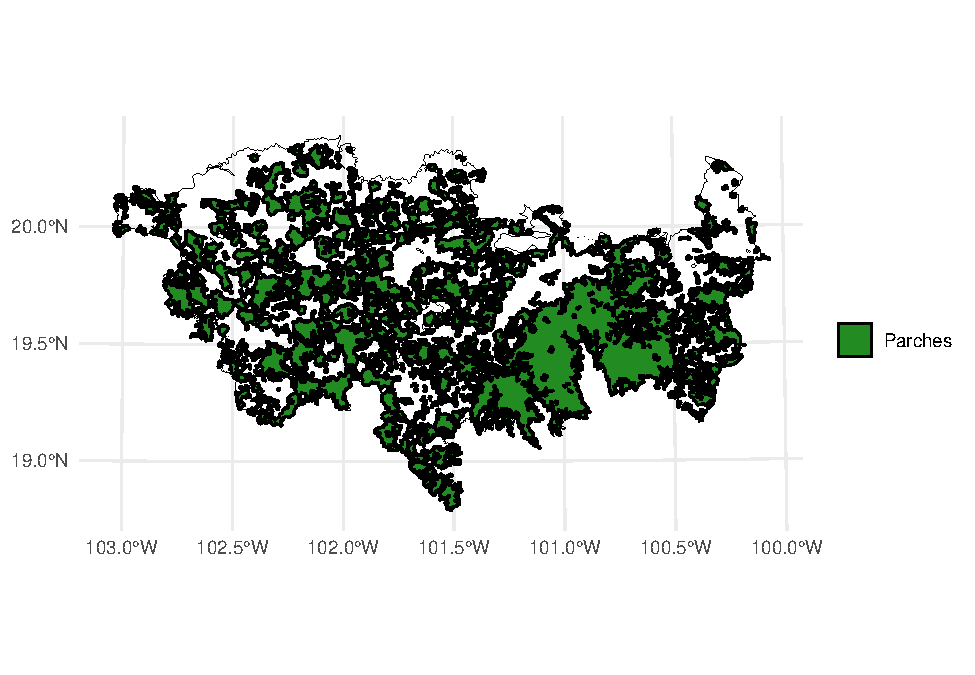
\includegraphics[keepaspectratio]{02-Fragmentacion_files/figure-latex/unnamed-chunk-4-1.pdf}}

En caso de necesitar abrir otro vector (e.g., .shp, .gpkg) necesitan usar la fución \texttt{read\_sf()} del paquete \texttt{sf}, la función \texttt{shapefile()} del paquete \texttt{raster}, o la funcion \texttt{vect()} del paquete \texttt{terra}.

Para abrirlo solo necesitan colocar la dirección de su archivo, el nombre y la extensión, ejemplo:

\begin{itemize}
\item
  \texttt{vegetation\_patches\ \textless{}-\ sf::read\_sf("D:/Datos/vegetation\_patches.shp")}
\item
  \texttt{vegetation\_patches\ \textless{}-\ raster::shapefile("D:/Datos/vegetation\_patches.shp")}
\item
  \texttt{vegetation\_patches\ \textless{}-\ terra::vect("D:/Datos/vegetation\_patches.shp")}
\end{itemize}

Para definir el borde usaremos una distancia de 500 m a partir del límite de los parches (Haddad et al.~2015).

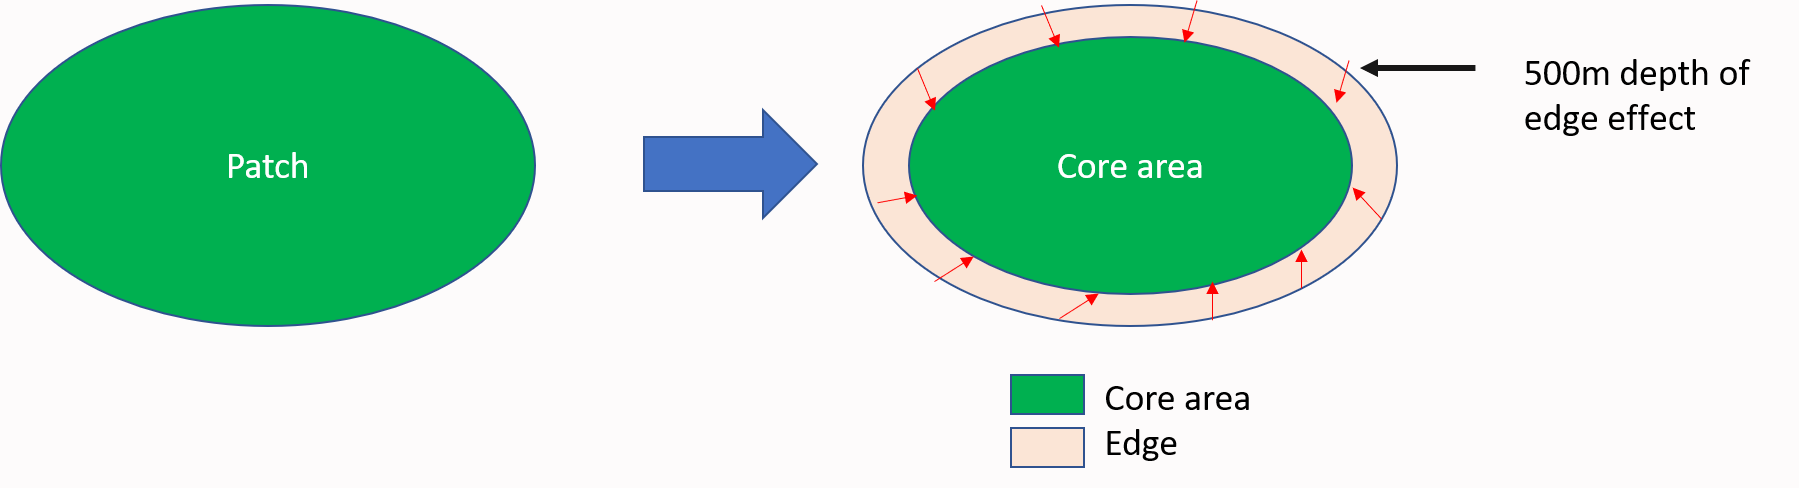
\includegraphics[width=5.23958in,height=\textheight,keepaspectratio]{Imagen1.png}

\section{Funcion}\label{funcion}

\begin{Shaded}
\begin{Highlighting}[]
\FunctionTok{MK\_Fragmentation}\NormalTok{(}
  \AttributeTok{nodes =} \ConstantTok{NULL}\NormalTok{,}
  \AttributeTok{edge\_distance =} \DecValTok{500}\NormalTok{,}
  \AttributeTok{min\_node\_area =} \DecValTok{100}\NormalTok{,}
  \AttributeTok{landscape\_area =} \ConstantTok{NULL}\NormalTok{,}
  \AttributeTok{area\_unit =} \StringTok{"ha"}\NormalTok{,}
  \AttributeTok{perimeter\_unit =} \StringTok{"km"}\NormalTok{,}
  \AttributeTok{plot =} \ConstantTok{FALSE}\NormalTok{,}
  \AttributeTok{write =} \ConstantTok{NULL}
\NormalTok{)}
\end{Highlighting}
\end{Shaded}

Los argumento de la función que usaremos son:

\begin{itemize}
\tightlist
\item
  \emph{nodes} = objeto con los parches,
\item
  \emph{edge\_distance} = profundidad del efecto de borde.
\item
  \emph{min\_node\_area} = Área mínima del nodo utilizada para calcular el número de nodos con un área menor a la proporcionada. Por defecto igual a 100 km² (Haddad et al.~2015).
\item
  \emph{landscape\_area} = Área total del paisaje de estudio (opcional). Si se deja como NULL, se utilizará el área total de los nodos. La unidad de área debe ser igual a la seleccionada en el párametro \emph{area\_unit}.
\item
  \emph{area\_unit} = Puedes establecer una unidad de área (por ejemplo, ``km2'', ``cm2'', ``m2'', ``ha''; ver unit\_convert). Por defecto es kilómetros cuadrados ``km2''.
\item
  \emph{perimeter\_unit} = Puedes establecer una unidad de perímetro (por ejemplo, ``km'', ``cm'', ``m'', ``ha''; ver unit\_convert). Por defecto es kilómetros ``km''.
\item
  \emph{plot} = Genera histogramas básicos y un mapa de área núcleo - borde.
\item
  \emph{write} = Guarda la tabla (estadísticas del paisaje), el objeto sf (estadísticas de parches/nodos) y las gráficas. Es necesario especificar la ruta y el prefijo. Por ejemplo, para guardar en la ruta ``C:/Folder'' con el prefijo ``Fragmentation'': ``C:/Folder/Fragmentation''
\end{itemize}

\begin{Shaded}
\begin{Highlighting}[]
\FunctionTok{MK\_Fragmentation}\NormalTok{()}
\end{Highlighting}
\end{Shaded}

\section{Ejercicio 1}\label{ejercicio-1}

Estimamos el área del paisaje de estudio.

\begin{Shaded}
\begin{Highlighting}[]
\NormalTok{area\_paisaje }\OtherTok{\textless{}{-}} \FunctionTok{st\_area}\NormalTok{(paisaje) }
\NormalTok{area\_paisaje }\OtherTok{\textless{}{-}} \FunctionTok{unit\_convert}\NormalTok{(area\_paisaje, }\StringTok{"m2"}\NormalTok{, }\StringTok{"ha"}\NormalTok{) }
\end{Highlighting}
\end{Shaded}

Aplicamos la función.

\begin{Shaded}
\begin{Highlighting}[]
\NormalTok{Fragmentacion }\OtherTok{\textless{}{-}} \FunctionTok{MK\_Fragmentation}\NormalTok{(}\AttributeTok{nodes =}\NormalTok{ habitat\_nodes, }
                                  \AttributeTok{edge\_distance =} \DecValTok{500}\NormalTok{,}
                                  \AttributeTok{min\_node\_area =} \DecValTok{100}\NormalTok{,}
                                  \AttributeTok{landscape\_area =}\NormalTok{ area\_paisaje,}
                                  \AttributeTok{area\_unit =} \StringTok{"ha"}\NormalTok{,}
                                  \AttributeTok{perimeter\_unit =} \StringTok{"km"}\NormalTok{,}
                                  \AttributeTok{plot =} \ConstantTok{TRUE}\NormalTok{)}
\end{Highlighting}
\end{Shaded}

\pandocbounded{\includegraphics[keepaspectratio]{02-Fragmentacion_files/figure-latex/unnamed-chunk-8-1.pdf}} \pandocbounded{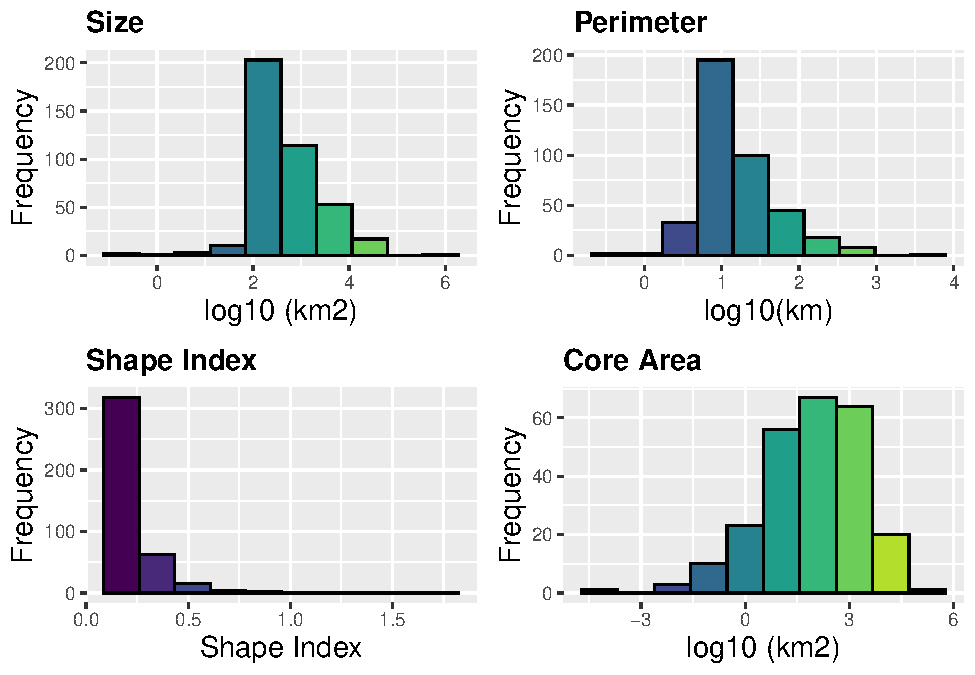
\includegraphics[keepaspectratio]{02-Fragmentacion_files/figure-latex/unnamed-chunk-8-2.pdf}}

\subsection{Estadisticos a nivel de parche}\label{estadisticos-a-nivel-de-parche}

El primer resultado ``Patch statistics shapefile'' es un shapefile con estadísticos de fragmentación a nivel de parche.

\begin{Shaded}
\begin{Highlighting}[]
\NormalTok{Fragmentacion}\SpecialCharTok{$}\StringTok{\textasciigrave{}}\AttributeTok{Patch statistics shapefile}\StringTok{\textasciigrave{}}
\CommentTok{\#\textgreater{} Simple feature collection with 404 features and 9 fields}
\CommentTok{\#\textgreater{} Geometry type: POLYGON}
\CommentTok{\#\textgreater{} Dimension:     XY}
\CommentTok{\#\textgreater{} Bounding box:  xmin: {-}108954 ymin: 2025032 xmax: 202330.2 ymax: 2198936}
\CommentTok{\#\textgreater{} Projected CRS: NAD\_1927\_Albers}
\CommentTok{\#\textgreater{} First 10 features:}
\CommentTok{\#\textgreater{}    Id       Area        CA CAPercent Perimeter EdgePercent}
\CommentTok{\#\textgreater{} 1   1    85.8368     0.000    0.0000     5.989    100.0000}
\CommentTok{\#\textgreater{} 2   2   220.2168     0.000    0.0000    11.346    100.0000}
\CommentTok{\#\textgreater{} 3   3 11019.9668  5337.795   48.4375   184.969     51.5625}
\CommentTok{\#\textgreater{} 4   4   121.0018     0.000    0.0000     6.974    100.0000}
\CommentTok{\#\textgreater{} 5   5   184.7226     0.000    0.0000    14.452    100.0000}
\CommentTok{\#\textgreater{} 6   6    26.3052     0.000    0.0000     4.685    100.0000}
\CommentTok{\#\textgreater{} 7   7    43.4931     0.000    0.0000     6.066    100.0000}
\CommentTok{\#\textgreater{} 8   8    57.5414     0.000    0.0000     8.119    100.0000}
\CommentTok{\#\textgreater{} 9   9   203.4670     0.000    0.0000    14.309    100.0000}
\CommentTok{\#\textgreater{} 10 10 29440.4346 12326.275   41.8685   444.203     58.1315}
\CommentTok{\#\textgreater{}       PARA ShapeIndex   FRAC                       geometry}
\CommentTok{\#\textgreater{} 1  14.3324     0.1824 0.8040 POLYGON ((54911.05 2035815,...}
\CommentTok{\#\textgreater{} 2  19.4092     0.2157 0.9005 POLYGON ((44591.28 2042209,...}
\CommentTok{\#\textgreater{} 3  59.5774     0.4971 1.1217 POLYGON ((46491.11 2042467,...}
\CommentTok{\#\textgreater{} 4  17.3504     0.1788 0.8100 POLYGON ((54944.49 2048163,...}
\CommentTok{\#\textgreater{} 5  12.7818     0.3000 1.0235 POLYGON ((80094.28 2064140,...}
\CommentTok{\#\textgreater{} 6   5.6148     0.2577 0.9446 POLYGON ((69205.24 2066394,...}
\CommentTok{\#\textgreater{} 7   7.1700     0.2595 0.9557 POLYGON ((68554.2 2066632, ...}
\CommentTok{\#\textgreater{} 8   7.0873     0.3019 1.0335 POLYGON ((69995.53 2066880,...}
\CommentTok{\#\textgreater{} 9  14.2195     0.2830 1.0012 POLYGON ((79368.68 2067324,...}
\CommentTok{\#\textgreater{} 10 66.2770     0.7303 1.1849 POLYGON ((23378.32 2067554,...}
\end{Highlighting}
\end{Shaded}

Son espacialmente explicitos y podemos visualizarlos con librerias como ggplot2

\begin{itemize}
\tightlist
\item
  \% de área núcleo:
\end{itemize}

\begin{Shaded}
\begin{Highlighting}[]
\FunctionTok{ggplot}\NormalTok{() }\SpecialCharTok{+}  
  \FunctionTok{geom\_sf}\NormalTok{(}\AttributeTok{data =}\NormalTok{ paisaje, }\FunctionTok{aes}\NormalTok{(}\AttributeTok{color =} \StringTok{"Study area"}\NormalTok{), }\AttributeTok{fill =} \ConstantTok{NA}\NormalTok{, }\AttributeTok{color =} \StringTok{"black"}\NormalTok{) }\SpecialCharTok{+}
  \FunctionTok{geom\_sf}\NormalTok{(}\AttributeTok{data =}\NormalTok{ Fragmentacion}\SpecialCharTok{$}\StringTok{\textasciigrave{}}\AttributeTok{Patch statistics shapefile}\StringTok{\textasciigrave{}}\NormalTok{, }\FunctionTok{aes}\NormalTok{(}\AttributeTok{fill =}\NormalTok{ CAPercent), }\AttributeTok{color =} \StringTok{"black"}\NormalTok{, }\AttributeTok{size =} \FloatTok{0.1}\NormalTok{) }\SpecialCharTok{+}
  \FunctionTok{scale\_fill\_distiller}\NormalTok{(}
    \AttributeTok{palette =} \StringTok{"RdYlGn"}\NormalTok{,}
    \AttributeTok{direction =} \DecValTok{1}\NormalTok{, }
    \AttributeTok{name =} \StringTok{"\% Área Núcleo"}
\NormalTok{  ) }\SpecialCharTok{+}
  \FunctionTok{theme\_minimal}\NormalTok{() }\SpecialCharTok{+}
  \FunctionTok{labs}\NormalTok{(}
    \AttributeTok{title =} \StringTok{"Fragmentación a nivel de parche"}\NormalTok{,}
    \AttributeTok{fill =} \StringTok{"\% Área Núcleo"}
\NormalTok{  ) }\SpecialCharTok{+}
  \FunctionTok{theme}\NormalTok{(}
    \AttributeTok{legend.position =} \StringTok{"right"}\NormalTok{,}
    \AttributeTok{plot.title =} \FunctionTok{element\_text}\NormalTok{(}\AttributeTok{hjust =} \FloatTok{0.5}\NormalTok{)}
\NormalTok{  )}
\end{Highlighting}
\end{Shaded}

\pandocbounded{\includegraphics[keepaspectratio]{02-Fragmentacion_files/figure-latex/unnamed-chunk-10-1.pdf}}

\begin{itemize}
\tightlist
\item
  \% de borde
\end{itemize}

\begin{Shaded}
\begin{Highlighting}[]
\FunctionTok{ggplot}\NormalTok{() }\SpecialCharTok{+}  
  \FunctionTok{geom\_sf}\NormalTok{(}\AttributeTok{data =}\NormalTok{ paisaje, }\FunctionTok{aes}\NormalTok{(}\AttributeTok{color =} \StringTok{"Study area"}\NormalTok{), }\AttributeTok{fill =} \ConstantTok{NA}\NormalTok{, }\AttributeTok{color =} \StringTok{"black"}\NormalTok{) }\SpecialCharTok{+}
  \FunctionTok{geom\_sf}\NormalTok{(}\AttributeTok{data =}\NormalTok{ Fragmentacion}\SpecialCharTok{$}\StringTok{\textasciigrave{}}\AttributeTok{Patch statistics shapefile}\StringTok{\textasciigrave{}}\NormalTok{, }\FunctionTok{aes}\NormalTok{(}\AttributeTok{fill =}\NormalTok{ EdgePercent), }\AttributeTok{color =} \StringTok{"black"}\NormalTok{, }\AttributeTok{size =} \FloatTok{0.1}\NormalTok{) }\SpecialCharTok{+}
  \FunctionTok{scale\_fill\_distiller}\NormalTok{(}
    \AttributeTok{palette =} \StringTok{"RdYlGn"}\NormalTok{,}
    \AttributeTok{direction =} \SpecialCharTok{{-}}\DecValTok{1}\NormalTok{, }
    \AttributeTok{name =} \StringTok{"\% Borde"}
\NormalTok{  ) }\SpecialCharTok{+}
  \FunctionTok{theme\_minimal}\NormalTok{() }\SpecialCharTok{+}
  \FunctionTok{labs}\NormalTok{(}
    \AttributeTok{title =} \StringTok{"Fragmentación a nivel de parche"}\NormalTok{,}
    \AttributeTok{fill =} \StringTok{"\% Borde"}
\NormalTok{  ) }\SpecialCharTok{+}
  \FunctionTok{theme}\NormalTok{(}
    \AttributeTok{legend.position =} \StringTok{"right"}\NormalTok{,}
    \AttributeTok{plot.title =} \FunctionTok{element\_text}\NormalTok{(}\AttributeTok{hjust =} \FloatTok{0.5}\NormalTok{)}
\NormalTok{  )}
\end{Highlighting}
\end{Shaded}

\pandocbounded{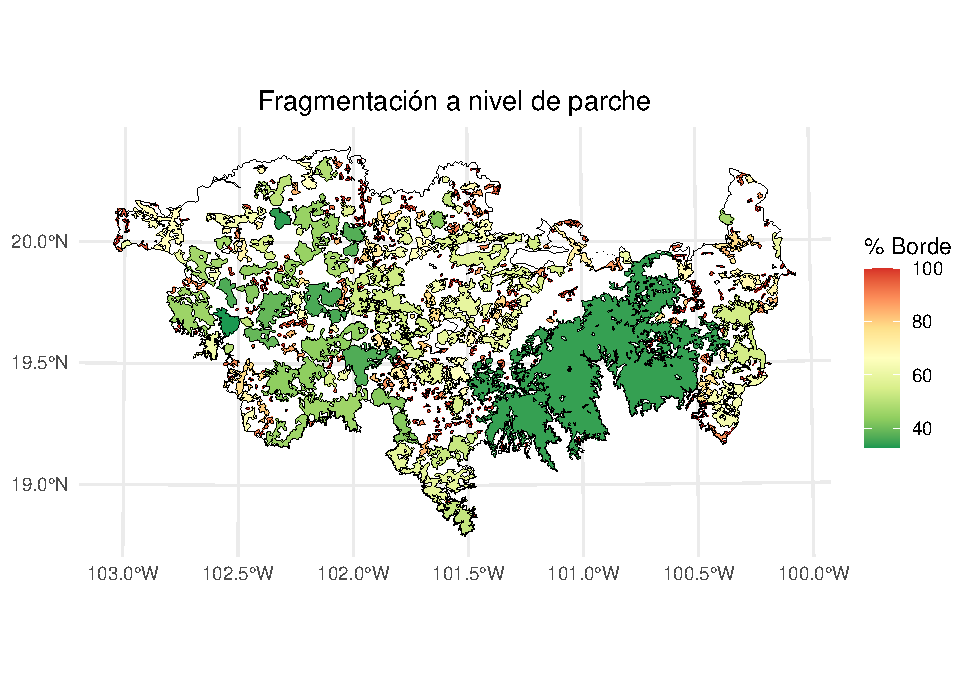
\includegraphics[keepaspectratio]{02-Fragmentacion_files/figure-latex/unnamed-chunk-11-1.pdf}}

\begin{itemize}
\tightlist
\item
  Perimeter
\end{itemize}

\begin{Shaded}
\begin{Highlighting}[]
\FunctionTok{ggplot}\NormalTok{() }\SpecialCharTok{+}  
  \FunctionTok{geom\_sf}\NormalTok{(}\AttributeTok{data =}\NormalTok{ paisaje, }\FunctionTok{aes}\NormalTok{(}\AttributeTok{color =} \StringTok{"Study area"}\NormalTok{), }\AttributeTok{fill =} \ConstantTok{NA}\NormalTok{, }\AttributeTok{color =} \StringTok{"black"}\NormalTok{) }\SpecialCharTok{+}
  \FunctionTok{geom\_sf}\NormalTok{(}\AttributeTok{data =}\NormalTok{ Fragmentacion}\SpecialCharTok{$}\StringTok{\textasciigrave{}}\AttributeTok{Patch statistics shapefile}\StringTok{\textasciigrave{}}\NormalTok{, }\FunctionTok{aes}\NormalTok{(}\AttributeTok{fill =}\NormalTok{ Perimeter), }\AttributeTok{color =} \StringTok{"black"}\NormalTok{, }\AttributeTok{size =} \FloatTok{0.1}\NormalTok{) }\SpecialCharTok{+}
  \FunctionTok{scale\_fill\_distiller}\NormalTok{(}
    \AttributeTok{palette =} \StringTok{"RdYlGn"}\NormalTok{,}
    \AttributeTok{direction =} \SpecialCharTok{{-}}\DecValTok{1}\NormalTok{, }
    \AttributeTok{name =} \StringTok{"Perímetro"}
\NormalTok{  ) }\SpecialCharTok{+}
  \FunctionTok{theme\_minimal}\NormalTok{() }\SpecialCharTok{+}
  \FunctionTok{labs}\NormalTok{(}
    \AttributeTok{title =} \StringTok{"Fragmentación a nivel de parche"}\NormalTok{,}
    \AttributeTok{fill =} \StringTok{"Perímetro"}
\NormalTok{  ) }\SpecialCharTok{+}
  \FunctionTok{theme}\NormalTok{(}
    \AttributeTok{legend.position =} \StringTok{"right"}\NormalTok{,}
    \AttributeTok{plot.title =} \FunctionTok{element\_text}\NormalTok{(}\AttributeTok{hjust =} \FloatTok{0.5}\NormalTok{)}
\NormalTok{  )}
\end{Highlighting}
\end{Shaded}

\pandocbounded{\includegraphics[keepaspectratio]{02-Fragmentacion_files/figure-latex/unnamed-chunk-12-1.pdf}}

\begin{itemize}
\tightlist
\item
  Perimeter-Area Ratio
\end{itemize}

\begin{Shaded}
\begin{Highlighting}[]
\FunctionTok{ggplot}\NormalTok{() }\SpecialCharTok{+}  
  \FunctionTok{geom\_sf}\NormalTok{(}\AttributeTok{data =}\NormalTok{ paisaje, }\FunctionTok{aes}\NormalTok{(}\AttributeTok{color =} \StringTok{"Study area"}\NormalTok{), }\AttributeTok{fill =} \ConstantTok{NA}\NormalTok{, }\AttributeTok{color =} \StringTok{"black"}\NormalTok{) }\SpecialCharTok{+}
  \FunctionTok{geom\_sf}\NormalTok{(}\AttributeTok{data =}\NormalTok{ Fragmentacion}\SpecialCharTok{$}\StringTok{\textasciigrave{}}\AttributeTok{Patch statistics shapefile}\StringTok{\textasciigrave{}}\NormalTok{, }\FunctionTok{aes}\NormalTok{(}\AttributeTok{fill =}\NormalTok{ PARA), }\AttributeTok{color =} \StringTok{"black"}\NormalTok{, }\AttributeTok{size =} \FloatTok{0.1}\NormalTok{) }\SpecialCharTok{+}
  \FunctionTok{scale\_fill\_distiller}\NormalTok{(}
    \AttributeTok{palette =} \StringTok{"RdYlGn"}\NormalTok{,}
    \AttributeTok{direction =} \SpecialCharTok{{-}}\DecValTok{1}\NormalTok{, }
    \AttributeTok{name =} \StringTok{"PARA"}
\NormalTok{  ) }\SpecialCharTok{+}
  \FunctionTok{theme\_minimal}\NormalTok{() }\SpecialCharTok{+}
  \FunctionTok{labs}\NormalTok{(}
    \AttributeTok{title =} \StringTok{"Fragmentación a nivel de parche"}\NormalTok{,}
    \AttributeTok{fill =} \StringTok{"PARA"}
\NormalTok{  ) }\SpecialCharTok{+}
  \FunctionTok{theme}\NormalTok{(}
    \AttributeTok{legend.position =} \StringTok{"right"}\NormalTok{,}
    \AttributeTok{plot.title =} \FunctionTok{element\_text}\NormalTok{(}\AttributeTok{hjust =} \FloatTok{0.5}\NormalTok{)}
\NormalTok{  )}
\end{Highlighting}
\end{Shaded}

\pandocbounded{\includegraphics[keepaspectratio]{02-Fragmentacion_files/figure-latex/unnamed-chunk-13-1.pdf}}

\begin{itemize}
\tightlist
\item
  Shape Index
\end{itemize}

\begin{Shaded}
\begin{Highlighting}[]
\FunctionTok{ggplot}\NormalTok{() }\SpecialCharTok{+}  
  \FunctionTok{geom\_sf}\NormalTok{(}\AttributeTok{data =}\NormalTok{ paisaje, }\FunctionTok{aes}\NormalTok{(}\AttributeTok{color =} \StringTok{"Study area"}\NormalTok{), }\AttributeTok{fill =} \ConstantTok{NA}\NormalTok{, }\AttributeTok{color =} \StringTok{"black"}\NormalTok{) }\SpecialCharTok{+}
  \FunctionTok{geom\_sf}\NormalTok{(}\AttributeTok{data =}\NormalTok{ Fragmentacion}\SpecialCharTok{$}\StringTok{\textasciigrave{}}\AttributeTok{Patch statistics shapefile}\StringTok{\textasciigrave{}}\NormalTok{, }\FunctionTok{aes}\NormalTok{(}\AttributeTok{fill =}\NormalTok{ ShapeIndex), }\AttributeTok{color =} \StringTok{"black"}\NormalTok{, }\AttributeTok{size =} \FloatTok{0.1}\NormalTok{) }\SpecialCharTok{+}
  \FunctionTok{scale\_fill\_distiller}\NormalTok{(}
    \AttributeTok{palette =} \StringTok{"PiYG"}\NormalTok{,}
    \AttributeTok{direction =} \SpecialCharTok{{-}}\DecValTok{1}\NormalTok{, }
    \AttributeTok{name =} \StringTok{"Shape Index"}
\NormalTok{  ) }\SpecialCharTok{+}
  \FunctionTok{theme\_minimal}\NormalTok{() }\SpecialCharTok{+}
  \FunctionTok{labs}\NormalTok{(}
    \AttributeTok{title =} \StringTok{"Fragmentación a nivel de parche"}\NormalTok{,}
    \AttributeTok{fill =} \StringTok{"Shape Index"}
\NormalTok{  ) }\SpecialCharTok{+}
  \FunctionTok{theme}\NormalTok{(}
    \AttributeTok{legend.position =} \StringTok{"right"}\NormalTok{,}
    \AttributeTok{plot.title =} \FunctionTok{element\_text}\NormalTok{(}\AttributeTok{hjust =} \FloatTok{0.5}\NormalTok{)}
\NormalTok{  )}
\end{Highlighting}
\end{Shaded}

\pandocbounded{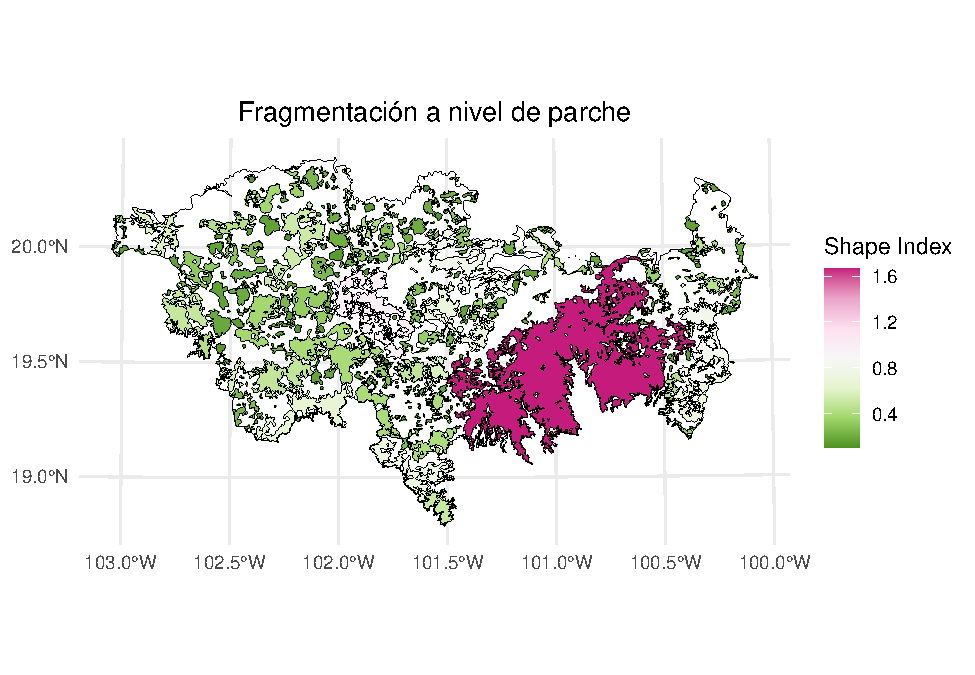
\includegraphics[keepaspectratio]{02-Fragmentacion_files/figure-latex/unnamed-chunk-14-1.pdf}}

\begin{itemize}
\tightlist
\item
  Fractal Dimension Index
\end{itemize}

\begin{Shaded}
\begin{Highlighting}[]
\FunctionTok{ggplot}\NormalTok{() }\SpecialCharTok{+}  
  \FunctionTok{geom\_sf}\NormalTok{(}\AttributeTok{data =}\NormalTok{ paisaje, }\FunctionTok{aes}\NormalTok{(}\AttributeTok{color =} \StringTok{"Study area"}\NormalTok{), }\AttributeTok{fill =} \ConstantTok{NA}\NormalTok{, }\AttributeTok{color =} \StringTok{"black"}\NormalTok{) }\SpecialCharTok{+}
  \FunctionTok{geom\_sf}\NormalTok{(}\AttributeTok{data =}\NormalTok{ Fragmentacion}\SpecialCharTok{$}\StringTok{\textasciigrave{}}\AttributeTok{Patch statistics shapefile}\StringTok{\textasciigrave{}}\NormalTok{, }\FunctionTok{aes}\NormalTok{(}\AttributeTok{fill =}\NormalTok{ FRAC), }\AttributeTok{color =} \StringTok{"black"}\NormalTok{, }\AttributeTok{size =} \FloatTok{0.1}\NormalTok{) }\SpecialCharTok{+}
  \FunctionTok{scale\_fill\_distiller}\NormalTok{(}
    \AttributeTok{palette =} \StringTok{"PiYG"}\NormalTok{,}
    \AttributeTok{direction =} \SpecialCharTok{{-}}\DecValTok{1}\NormalTok{, }
    \AttributeTok{name =} \StringTok{"FRAC"}
\NormalTok{  ) }\SpecialCharTok{+}
  \FunctionTok{theme\_minimal}\NormalTok{() }\SpecialCharTok{+}
  \FunctionTok{labs}\NormalTok{(}
    \AttributeTok{title =} \StringTok{"Fragmentación a nivel de parche"}\NormalTok{,}
    \AttributeTok{fill =} \StringTok{"FRAC"}
\NormalTok{  ) }\SpecialCharTok{+}
  \FunctionTok{theme}\NormalTok{(}
    \AttributeTok{legend.position =} \StringTok{"right"}\NormalTok{,}
    \AttributeTok{plot.title =} \FunctionTok{element\_text}\NormalTok{(}\AttributeTok{hjust =} \FloatTok{0.5}\NormalTok{)}
\NormalTok{  )}
\end{Highlighting}
\end{Shaded}

\pandocbounded{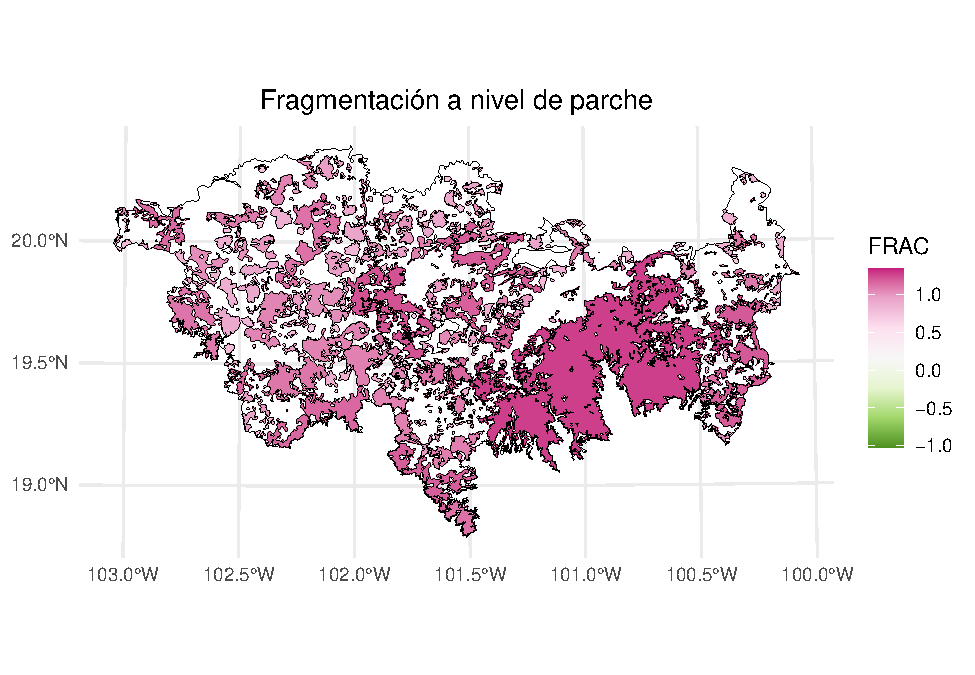
\includegraphics[keepaspectratio]{02-Fragmentacion_files/figure-latex/unnamed-chunk-15-1.pdf}}

\subsection{Estadísticos a nivel de paisaje}\label{estaduxedsticos-a-nivel-de-paisaje}

Los resultados se presentan a manera de una lista, el primer resultado se llama ``Summary landscape metrics (Viewer Panel)'' y tiene estadisticos de fragmentación a nivel de paisaje.

\begin{Shaded}
\begin{Highlighting}[]
\FunctionTok{class}\NormalTok{(Fragmentacion)}
\CommentTok{\#\textgreater{} [1] "list"}
\NormalTok{Fragmentacion}\SpecialCharTok{$}\StringTok{\textasciigrave{}}\AttributeTok{Summary landscape metrics (Viewer Panel)}\StringTok{\textasciigrave{}}
\end{Highlighting}
\end{Shaded}

Metric

Value

Patch area (ha)

1273573.9249

Number of patches

404.0000

Size (mean)

3152.4107

Patches \textless{} minimum patch area

40.0000

Patches \textless{} minimum patch area (\%)

0.1992

Total edge

17920.4740

Edge density

0.0141

Patch density

0.0146

Total Core Area (ha)

631595.3522

Cority

0.6064

Shape Index (mean)

0.2207

FRAC (mean)

0.8536

MESH (ha)

66572.5742

\pandocbounded{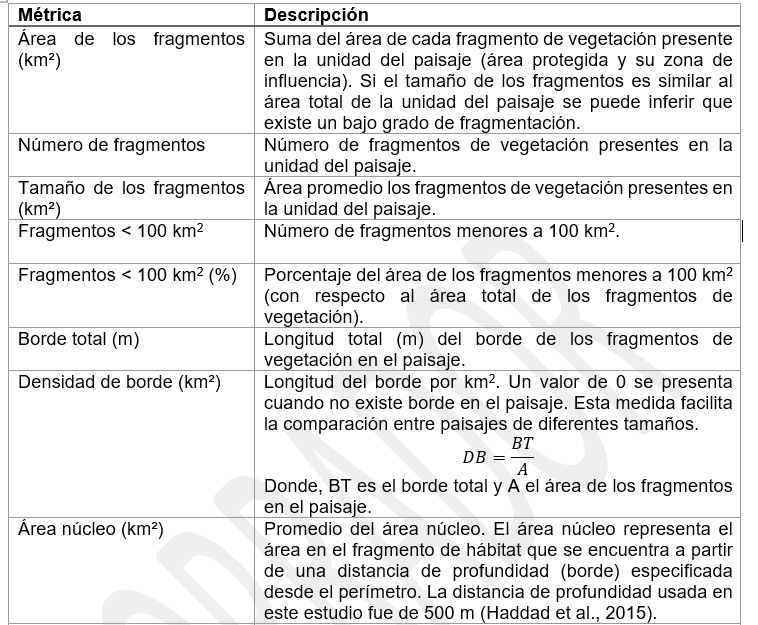
\includegraphics[keepaspectratio]{5.png}}\pandocbounded{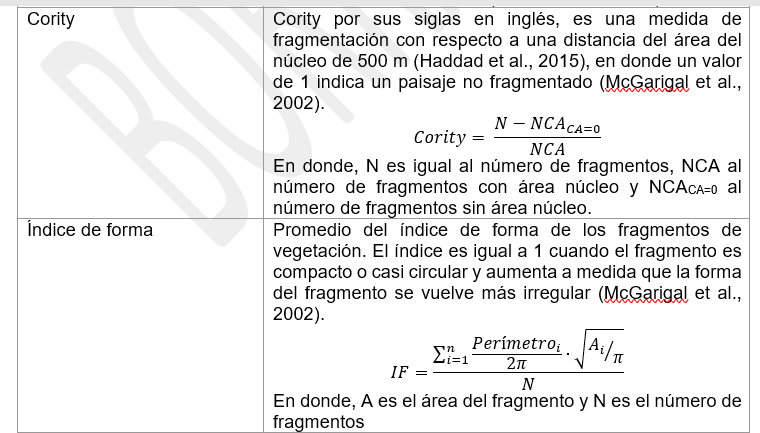
\includegraphics[keepaspectratio]{6.png}} \pandocbounded{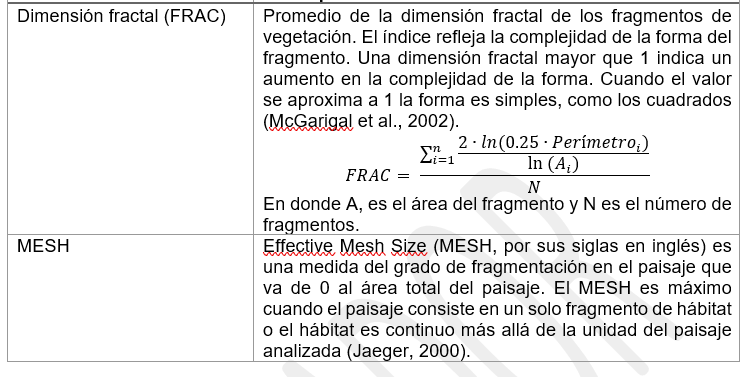
\includegraphics[keepaspectratio]{7.png}}

La densidad de malla efectiva (MESH) es una medida del grado en que el movimiento entre diferentes partes del paisaje se ve interrumpido por una Fragmentación. El índice MESH se ha popularizado debido a su facilidad de interpretación. Si conocemos el área de nuestro paisaje, entonces podemos estimar el porcentage de fragmentación:

\begin{Shaded}
\begin{Highlighting}[]
\NormalTok{mesh }\OtherTok{\textless{}{-}} \FunctionTok{as.data.frame}\NormalTok{(Fragmentacion[[}\DecValTok{1}\NormalTok{]])}
\NormalTok{mesh }\OtherTok{\textless{}{-}}\NormalTok{ mesh[}\DecValTok{13}\NormalTok{,}\DecValTok{2}\NormalTok{]}
\NormalTok{mesh\_porcentage }\OtherTok{\textless{}{-}}\NormalTok{  (area\_paisaje }\SpecialCharTok{{-}}\NormalTok{ mesh) }\SpecialCharTok{*} \DecValTok{100} \SpecialCharTok{/}\NormalTok{ area\_paisaje }
\NormalTok{mesh\_porcentage}
\CommentTok{\#\textgreater{} [1] 97.58915}
\end{Highlighting}
\end{Shaded}

\section{Ejercicio 2}\label{ejercicio-2}

Hagamos un loop en donde exploramos distintas distancias de profundidad del efecto borde.

\begin{Shaded}
\begin{Highlighting}[]
\CommentTok{\#Loop edge distance}
\FunctionTok{library}\NormalTok{(purrr)}
\NormalTok{Fragmentacion}\FloatTok{.2} \OtherTok{\textless{}{-}} \FunctionTok{map\_dfr}\NormalTok{(}\FunctionTok{seq}\NormalTok{(}\DecValTok{100}\NormalTok{, }\DecValTok{1000}\NormalTok{, }\DecValTok{100}\NormalTok{), }\ControlFlowTok{function}\NormalTok{(x)\{}
\NormalTok{  x}\FloatTok{.1} \OtherTok{\textless{}{-}} \FunctionTok{MK\_Fragmentation}\NormalTok{(}\AttributeTok{nodes =}\NormalTok{ habitat\_nodes, }
                          \AttributeTok{edge\_distance =}\NormalTok{ x, }\AttributeTok{plot =} \ConstantTok{FALSE}\NormalTok{)[[}\DecValTok{2}\NormalTok{]]}
\NormalTok{  CA }\OtherTok{\textless{}{-}} \FunctionTok{mean}\NormalTok{(x}\FloatTok{.1}\SpecialCharTok{$}\NormalTok{CAPercent)}
\NormalTok{  Edge }\OtherTok{\textless{}{-}} \FunctionTok{mean}\NormalTok{(x}\FloatTok{.1}\SpecialCharTok{$}\NormalTok{EdgePercent)}
\NormalTok{  x}\FloatTok{.2} \OtherTok{\textless{}{-}} \FunctionTok{rbind}\NormalTok{(}\FunctionTok{data.frame}\NormalTok{(}\StringTok{\textquotesingle{}Edge distance\textquotesingle{}} \OtherTok{=}\NormalTok{ x, }\AttributeTok{Type =} \StringTok{"Core Area"}\NormalTok{, }\AttributeTok{Percentage =}\NormalTok{ CA),}
                     \FunctionTok{data.frame}\NormalTok{(}\StringTok{\textquotesingle{}Edge distance\textquotesingle{}} \OtherTok{=}\NormalTok{ x, }\AttributeTok{Type =} \StringTok{"Edge"}\NormalTok{, }\AttributeTok{Percentage =}\NormalTok{ Edge))}
  \FunctionTok{return}\NormalTok{(x}\FloatTok{.2}\NormalTok{)}
\NormalTok{\}, }\AttributeTok{.progress =} \ConstantTok{TRUE}\NormalTok{)}


\NormalTok{Fragmentacion}\FloatTok{.2} 
\end{Highlighting}
\end{Shaded}

\begin{verbatim}
#>    Edge.distance      Type Percentage
#> 1            100 Core Area  65.761207
#> 2            100      Edge  34.238793
#> 3            200 Core Area  41.980654
#> 4            200      Edge  58.019346
#> 5            300 Core Area  26.853211
#> 6            300      Edge  73.146789
#> 7            400 Core Area  18.110913
#> 8            400      Edge  81.889087
#> 9            500 Core Area  12.863545
#> 10           500      Edge  87.136455
#> 11           600 Core Area   9.554117
#> 12           600      Edge  90.445883
#> 13           700 Core Area   7.347448
#> 14           700      Edge  92.652552
#> 15           800 Core Area   5.767296
#> 16           800      Edge  94.232704
#> 17           900 Core Area   4.564680
#> 18           900      Edge  95.435320
#> 19          1000 Core Area   3.633780
#> 20          1000      Edge  96.366220
\end{verbatim}

El porcentaje promedio de área núcleo (ausencia de efecto de borde) para todos los parches disminuye en más del 70\% cuando se considera un efecto de borde con una penetración de 1 km.

\begin{longtable}[]{@{}lc@{}}
\toprule\noalign{}
Distancia de profundidad & \%Área Núcleo \\
\midrule\noalign{}
\endhead
\bottomrule\noalign{}
\endlastfoot
100 & 65.76\% \\
500 & 12.86\% \\
1000 & 3.63\% \\
\end{longtable}

Podemos gráficar el promedio del porcentaje de área npucleo de los parches y el porcentaje del borde de los parches (\%área núcleo + \% de borde = 100\%).

\begin{Shaded}
\begin{Highlighting}[]
\FunctionTok{library}\NormalTok{(ggplot2)}
\FunctionTok{ggplot}\NormalTok{(Fragmentacion}\FloatTok{.2}\NormalTok{, }\FunctionTok{aes}\NormalTok{(}\AttributeTok{x=}\NormalTok{Edge.distance, }\AttributeTok{y=}\NormalTok{Percentage, }\AttributeTok{group=}\NormalTok{Type)) }\SpecialCharTok{+}
  \FunctionTok{geom\_line}\NormalTok{(}\FunctionTok{aes}\NormalTok{(}\AttributeTok{color=}\NormalTok{Type))}\SpecialCharTok{+}
  \FunctionTok{geom\_point}\NormalTok{(}\FunctionTok{aes}\NormalTok{(}\AttributeTok{color=}\NormalTok{Type))}\SpecialCharTok{+} \FunctionTok{ylim}\NormalTok{(}\DecValTok{0}\NormalTok{,}\DecValTok{100}\NormalTok{)}\SpecialCharTok{+}
  \FunctionTok{scale\_x\_continuous}\NormalTok{(}\StringTok{"Distancia"}\NormalTok{, }\AttributeTok{labels =} \FunctionTok{as.character}\NormalTok{(Fragmentacion}\FloatTok{.2}\SpecialCharTok{$}\NormalTok{Edge.distance), }\AttributeTok{breaks =}\NormalTok{ Fragmentacion}\FloatTok{.2}\SpecialCharTok{$}\NormalTok{Edge.distance)}\SpecialCharTok{+}
  \FunctionTok{scale\_color\_brewer}\NormalTok{(}\AttributeTok{palette=}\StringTok{"Dark2"}\NormalTok{)}\SpecialCharTok{+}
  \FunctionTok{theme\_classic}\NormalTok{()}
\end{Highlighting}
\end{Shaded}

\pandocbounded{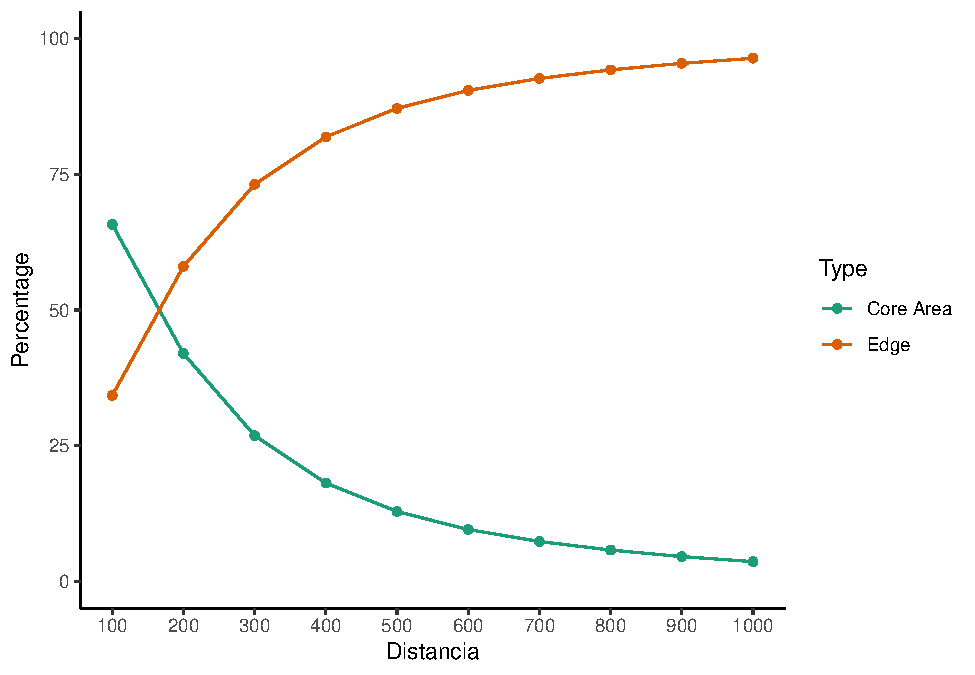
\includegraphics[keepaspectratio]{02-Fragmentacion_files/figure-latex/unnamed-chunk-20-1.pdf}}

\section{Ejercicio 3}\label{ejercicio-3}

Ahora probemos los alcances de la función estimando el índice MESH sobre un grid.

Grid de 40 km2

\begin{Shaded}
\begin{Highlighting}[]
\NormalTok{Grid\_test }\OtherTok{\textless{}{-}} \FunctionTok{make\_grid}\NormalTok{(}\AttributeTok{x =}\NormalTok{ paisaje, }\AttributeTok{hexagonal =} \ConstantTok{FALSE}\NormalTok{,}
                  \AttributeTok{cell\_area =} \FunctionTok{unit\_convert}\NormalTok{(}\DecValTok{40}\NormalTok{, }\StringTok{"km2"}\NormalTok{, }\StringTok{"m2"}\NormalTok{),}
                  \AttributeTok{clip =} \ConstantTok{TRUE}\NormalTok{)}
\FunctionTok{plot}\NormalTok{(Grid\_test)}
\end{Highlighting}
\end{Shaded}

\pandocbounded{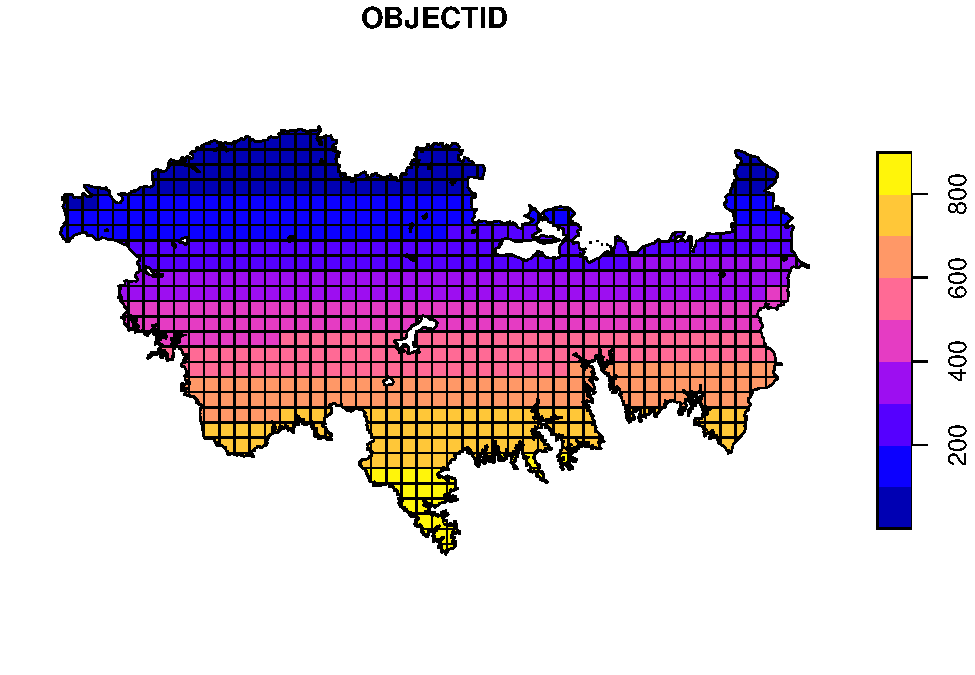
\includegraphics[keepaspectratio]{02-Fragmentacion_files/figure-latex/unnamed-chunk-21-1.pdf}}

Estimar MESH usando un loop sencillo tipo \texttt{for()}

\begin{Shaded}
\begin{Highlighting}[]
\CommentTok{\#Variable dummy}
\NormalTok{Grid\_test}\SpecialCharTok{$}\NormalTok{MESH }\OtherTok{\textless{}{-}} \DecValTok{0}
\end{Highlighting}
\end{Shaded}

\begin{Shaded}
\begin{Highlighting}[]

\ControlFlowTok{for}\NormalTok{(i }\ControlFlowTok{in} \DecValTok{1}\SpecialCharTok{:}\FunctionTok{nrow}\NormalTok{(test))\{}
  \FunctionTok{cat}\NormalTok{(}\FunctionTok{paste0}\NormalTok{(i, }\StringTok{" de "}\NormalTok{, }\FunctionTok{nrow}\NormalTok{(test)))}
\NormalTok{  grid.i }\OtherTok{\textless{}{-}}\NormalTok{ Grid\_test[i,]}
\NormalTok{  nodes.i }\OtherTok{\textless{}{-}} \FunctionTok{suppressWarnings}\NormalTok{(}\FunctionTok{st\_intersection}\NormalTok{(habitat\_nodes, grid.i))}
  
  \ControlFlowTok{if}\NormalTok{(}\FunctionTok{nrow}\NormalTok{(nodes.i) }\SpecialCharTok{\textgreater{}} \DecValTok{0}\NormalTok{)\{}
\NormalTok{    area\_paisaje.i }\OtherTok{\textless{}{-}} \FunctionTok{st\_area}\NormalTok{(grid.i)}
\NormalTok{    area\_paisaje.i }\OtherTok{\textless{}{-}} \FunctionTok{unit\_convert}\NormalTok{(area\_paisaje.i, }\StringTok{"m2"}\NormalTok{, }\StringTok{"ha"}\NormalTok{)}
\NormalTok{    Fragmentacion.i }\OtherTok{\textless{}{-}} \FunctionTok{MK\_Fragmentation}\NormalTok{(}\AttributeTok{nodes =}\NormalTok{ nodes.i, }
                                      \AttributeTok{edge\_distance =} \DecValTok{500}\NormalTok{,}
                                      \AttributeTok{min\_node\_area =} \DecValTok{100}\NormalTok{,}
                                      \AttributeTok{landscape\_area =}\NormalTok{ ,}
                                      \AttributeTok{area\_unit =} \StringTok{"ha"}\NormalTok{,}
                                      \AttributeTok{perimeter\_unit =} \StringTok{"km"}\NormalTok{,}
                                      \AttributeTok{plot =} \ConstantTok{FALSE}\NormalTok{)}
\NormalTok{    mesh }\OtherTok{\textless{}{-}} \FunctionTok{as.data.frame}\NormalTok{(Fragmentacion.i[[}\DecValTok{1}\NormalTok{]])}
\NormalTok{    mesh }\OtherTok{\textless{}{-}}\NormalTok{ mesh[}\DecValTok{13}\NormalTok{,}\DecValTok{2}\NormalTok{]}
\NormalTok{    mesh\_porcentage }\OtherTok{\textless{}{-}}\NormalTok{  (area\_paisaje.i }\SpecialCharTok{{-}}\NormalTok{ mesh)}\SpecialCharTok{*}\DecValTok{100}\SpecialCharTok{/}\NormalTok{area\_paisaje.i }
\NormalTok{    Grid\_test}\SpecialCharTok{$}\NormalTok{MESH[i] }\OtherTok{\textless{}{-}}\NormalTok{ mesh\_porcentage}
\NormalTok{  \} }\ControlFlowTok{else}\NormalTok{ \{}
\NormalTok{    Grid\_test}\SpecialCharTok{$}\NormalTok{MESH[i] }\OtherTok{\textless{}{-}} \DecValTok{100}
\NormalTok{  \}}
\NormalTok{\}}
\end{Highlighting}
\end{Shaded}

Lo podemos visualizar con \texttt{ggplot2}

\begin{Shaded}
\begin{Highlighting}[]
\FunctionTok{ggplot}\NormalTok{() }\SpecialCharTok{+}  
  \FunctionTok{geom\_sf}\NormalTok{(}\AttributeTok{data =}\NormalTok{ paisaje, }\FunctionTok{aes}\NormalTok{(}\AttributeTok{color =} \StringTok{"Study area"}\NormalTok{), }\AttributeTok{fill =} \ConstantTok{NA}\NormalTok{, }\AttributeTok{color =} \StringTok{"black"}\NormalTok{) }\SpecialCharTok{+}
  \FunctionTok{geom\_sf}\NormalTok{(}\AttributeTok{data =}\NormalTok{ Grid\_test, }\FunctionTok{aes}\NormalTok{(}\AttributeTok{fill =}\NormalTok{ MESH), }\AttributeTok{color =} \StringTok{"black"}\NormalTok{, }\AttributeTok{size =} \FloatTok{0.1}\NormalTok{) }\SpecialCharTok{+}
  \FunctionTok{scale\_fill\_distiller}\NormalTok{(}
    \AttributeTok{palette =} \StringTok{"RdYlGn"}\NormalTok{,}
    \AttributeTok{direction =} \SpecialCharTok{{-}}\DecValTok{1}\NormalTok{, }
    \AttributeTok{name =} \StringTok{"\% Fragmentación"}
\NormalTok{  ) }\SpecialCharTok{+}
  \FunctionTok{theme\_minimal}\NormalTok{() }\SpecialCharTok{+}
  \FunctionTok{labs}\NormalTok{(}
    \AttributeTok{title =} \StringTok{"GRID fragmentación (MESH)"}\NormalTok{,}
    \AttributeTok{fill =} \StringTok{"\% Fragmentación"}
\NormalTok{  ) }\SpecialCharTok{+}
  \FunctionTok{theme}\NormalTok{(}
    \AttributeTok{legend.position =} \StringTok{"right"}\NormalTok{,}
    \AttributeTok{plot.title =} \FunctionTok{element\_text}\NormalTok{(}\AttributeTok{hjust =} \FloatTok{0.5}\NormalTok{)}
\NormalTok{  )}
\end{Highlighting}
\end{Shaded}

\pandocbounded{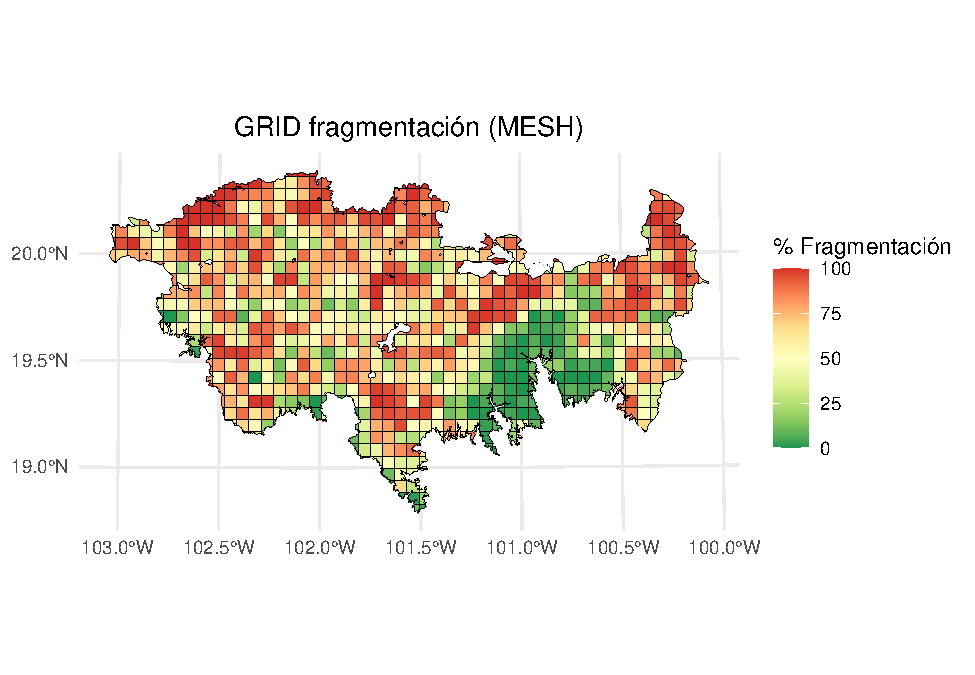
\includegraphics[keepaspectratio]{02-Fragmentacion_files/figure-latex/unnamed-chunk-25-1.pdf}}

\chapter{Índices de centralidad}\label{uxedndices-de-centralidad}

\section{Insumos y paquetes}\label{insumos-y-paquetes}

Seguimos trabajando con los mismos shapefiles de la sección anterior: habitat\_nodes y paisaje.

\begin{Shaded}
\begin{Highlighting}[]
\FunctionTok{library}\NormalTok{(ggplot2)}
\FunctionTok{library}\NormalTok{(sf)}
\FunctionTok{library}\NormalTok{(Makurhini)}
\FunctionTok{library}\NormalTok{(RColorBrewer)}
\end{Highlighting}
\end{Shaded}

\begin{verbatim}
#> Cargando paquete requerido: igraph
#> 
#> Adjuntando el paquete: 'igraph'
#> The following objects are masked from 'package:stats':
#> 
#>     decompose, spectrum
#> The following object is masked from 'package:base':
#> 
#>     union
#> Cargando paquete requerido: cppRouting
#> Linking to GEOS 3.13.0, GDAL 3.10.1, PROJ 9.5.1;
#> sf_use_s2() is TRUE
#> [1] 404
\end{verbatim}

\begin{Shaded}
\begin{Highlighting}[]
\FunctionTok{ggplot}\NormalTok{() }\SpecialCharTok{+}  
  \FunctionTok{geom\_sf}\NormalTok{(}\AttributeTok{data =}\NormalTok{ paisaje, }\FunctionTok{aes}\NormalTok{(}\AttributeTok{color =} \StringTok{"Study area"}\NormalTok{), }\AttributeTok{fill =} \ConstantTok{NA}\NormalTok{, }\AttributeTok{color =} \StringTok{"black"}\NormalTok{) }\SpecialCharTok{+}
  \FunctionTok{geom\_sf}\NormalTok{(}\AttributeTok{data =}\NormalTok{ habitat\_nodes, }\FunctionTok{aes}\NormalTok{(}\AttributeTok{color =} \StringTok{"Parches"}\NormalTok{), }\AttributeTok{fill =} \StringTok{"forestgreen"}\NormalTok{, }\AttributeTok{linewidth =} \FloatTok{0.5}\NormalTok{) }\SpecialCharTok{+}
  \FunctionTok{scale\_color\_manual}\NormalTok{(}\AttributeTok{name =} \StringTok{""}\NormalTok{, }\AttributeTok{values =} \StringTok{"black"}\NormalTok{)}\SpecialCharTok{+}
  \FunctionTok{theme\_minimal}\NormalTok{() }\SpecialCharTok{+}
  \FunctionTok{theme}\NormalTok{(}\AttributeTok{axis.title.x =} \FunctionTok{element\_blank}\NormalTok{(),}
        \AttributeTok{axis.title.y =} \FunctionTok{element\_blank}\NormalTok{())}
\end{Highlighting}
\end{Shaded}

\pandocbounded{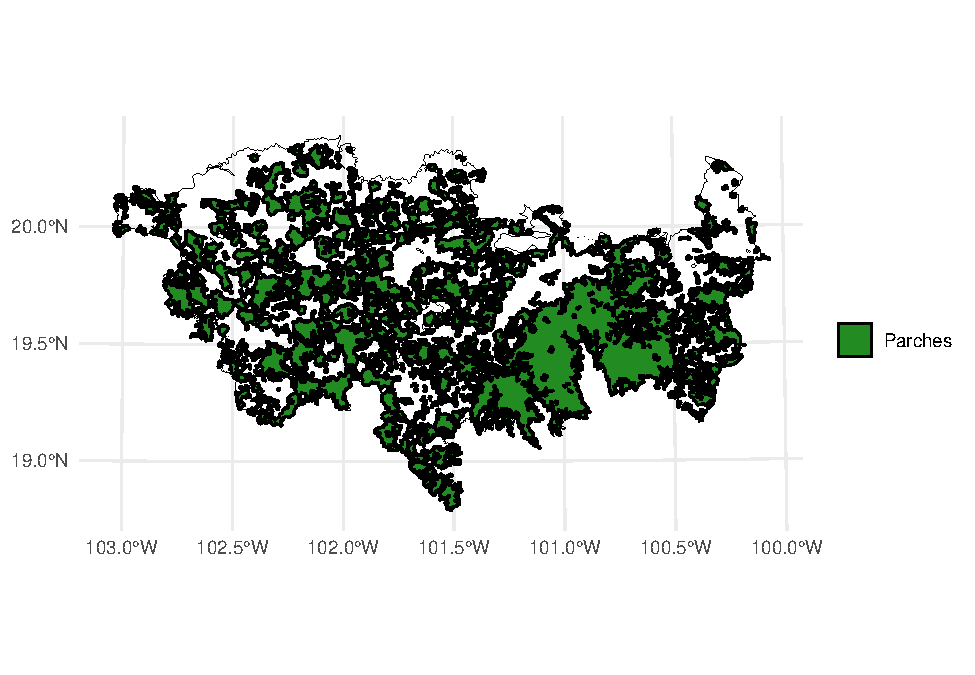
\includegraphics[keepaspectratio]{03-Centralidad_files/figure-latex/unnamed-chunk-3-1.pdf}}

En caso de necesitar abrir otro vector (e.g., .shp, .gpkg) necesitan usar la fución \texttt{read\_sf()} del paquete \texttt{sf}, la función \texttt{shapefile()} del paquete \texttt{raster}, o la funcion \texttt{vect()} del paquete \texttt{terra}.

Para abrirlo solo necesitan colocar la dirección de su archivo, el nombre y la extensión, ejemplo:

\begin{itemize}
\item
  \texttt{vegetation\_patches\ \textless{}-\ sf::read\_sf("D:/Datos/vegetation\_patches.shp")}
\item
  \texttt{vegetation\_patches\ \textless{}-\ raster::shapefile("D:/Datos/vegetation\_patches.shp")}
\item
  \texttt{vegetation\_patches\ \textless{}-\ terra::vect("D:/Datos/vegetation\_patches.shp")}
\end{itemize}

\section{MK\_RMCentrality()}\label{mk_rmcentrality}

La función \textbf{\texttt{MK\_RMCentrality()}} calcula medidas radiales (es decir, grado, fuerza, centralidad de vectores propios y centralidad de proximidad) y mediales (es decir, centralidad de interrelación, pertenencia a nodos y modularidad) de la centralidad de nodos para identificar, por ejemplo, stepping stones.

Las medidas o índices que estima son los siguientes:

\begin{itemize}
\tightlist
\item
  \textbf{Centralidad de Grado (degree)}: Cuántas conexiones directas tiene un nodo. Es como contar cuántos parches de hábitat están potencialmente conectados con el parche focal.
  \textbf{Más conexiones = mayor grado = más centralidad.}
\item
  \textbf{Centralidad de Grado (degree)}
\end{itemize}

\subsection{\texorpdfstring{1. Centralidad de Grado (\texttt{degree})}{1. Centralidad de Grado (degree)}}\label{centralidad-de-grado-degree}

\begin{quote}
Cuántas conexiones directas tiene un nodo.
\end{quote}

\begin{itemize}
\tightlist
\item
  Es como contar cuántos parches de hábitat o áreas protegidas están conectados con uno.
\item
  Más conexiones = mayor grado = más centralidad.
\end{itemize}

\subsection{\texorpdfstring{2. Fuerza (\texttt{strength}) \emph{(para redes ponderadas)}}{2. Fuerza (strength) (para redes ponderadas)}}\label{fuerza-strength-para-redes-ponderadas}

\begin{quote}
Como el grado, pero suma los \textbf{pesos} (o probabilidades) de los enlaces.
\end{quote}

\begin{itemize}
\tightlist
\item
  En lugar de solo contar conexiones, se suman qué tan \textbf{fuertes o probables} son (por ejemplo, probabilidad de dispersión).
\item
  Un nodo con pocas pero fuertes conexiones puede ser más central que uno con muchas pero débiles.
\end{itemize}

\subsection{\texorpdfstring{3. Centralidad de Vector Propio (\texttt{eigen})}{3. Centralidad de Vector Propio (eigen)}}\label{centralidad-de-vector-propio-eigen}

\begin{quote}
Mide cuán conectado está un nodo con \textbf{otros nodos importantes}.
\end{quote}

\begin{itemize}
\tightlist
\item
  Un nodo es importante si está conectado a otros nodos que también lo son.
\item
  Útil para detectar ``nodos influyentes'' en la red.
\end{itemize}

\subsection{\texorpdfstring{4. Centralidad de Cercanía (\texttt{close})}{4. Centralidad de Cercanía (close)}}\label{centralidad-de-cercanuxeda-close}

\begin{quote}
Qué tan cerca está un nodo de todos los demás.
\end{quote}

\begin{itemize}
\tightlist
\item
  Se calcula como el inverso de la suma de distancias a todos los demás nodos.
\item
  Los nodos con alta cercanía pueden \textbf{difundir o recibir información rápidamente}.
\end{itemize}

\begin{center}\rule{0.5\linewidth}{0.5pt}\end{center}

\subsection{Medidas Mediales (¿Quién está en medio o conecta otros nodos?)}\label{medidas-mediales-quiuxe9n-estuxe1-en-medio-o-conecta-otros-nodos}

\subsubsection{\texorpdfstring{5. Centralidad de Intermediación (\texttt{BWC})}{5. Centralidad de Intermediación (BWC)}}\label{centralidad-de-intermediaciuxf3n-bwc}

\begin{quote}
Cuántas veces un nodo se encuentra \textbf{en las rutas más cortas} entre otros nodos.
\end{quote}

\begin{itemize}
\tightlist
\item
  Nodos con alta intermediación actúan como puentes o \textbf{cuellos de botella}.
\item
  Muy importantes para la conectividad --- si se eliminan, pueden fragmentar la red.
\end{itemize}

\begin{center}\rule{0.5\linewidth}{0.5pt}\end{center}

\subsection{Detección de Comunidades (¿Quién pertenece al mismo grupo?)}\label{detecciuxf3n-de-comunidades-quiuxe9n-pertenece-al-mismo-grupo}

\subsubsection{\texorpdfstring{6. Caminatas Aleatorias Cortas (\texttt{memb.rw})}{6. Caminatas Aleatorias Cortas (memb.rw)}}\label{caminatas-aleatorias-cortas-memb.rw}

\begin{quote}
Agrupa nodos según la probabilidad de que una caminata aleatoria \textbf{permanezca dentro del grupo}.
\end{quote}

\begin{itemize}
\tightlist
\item
  Simula un animal moviéndose aleatoriamente por la red.
\item
  Detecta grupos \textbf{fuertemente conectados}.
\end{itemize}

\subsubsection{\texorpdfstring{7. Algoritmo de Louvain (\texttt{memb.louvain})}{7. Algoritmo de Louvain (memb.louvain)}}\label{algoritmo-de-louvain-memb.louvain}

\begin{quote}
Divide la red en comunidades para \textbf{maximizar la modularidad} (qué tan separados están los grupos).
\end{quote}

\begin{itemize}
\tightlist
\item
  Encuentra grupos donde los nodos están más conectados entre sí que con el resto.
\item
  Es rápido y muy usado en redes ecológicas grandes.
\end{itemize}

\begin{center}\rule{0.5\linewidth}{0.5pt}\end{center}

\subsection{La función}\label{la-funciuxf3n}

\begin{Shaded}
\begin{Highlighting}[]
\FunctionTok{MK\_RMCentrality}\NormalTok{(}
\NormalTok{  nodes,}
  \AttributeTok{distance =} \FunctionTok{list}\NormalTok{(}\AttributeTok{type =} \StringTok{"centroid"}\NormalTok{),}
  \AttributeTok{distance\_thresholds =} \ConstantTok{NULL}\NormalTok{,}
  \AttributeTok{binary =} \ConstantTok{TRUE}\NormalTok{,}
  \AttributeTok{probability =} \ConstantTok{NULL}\NormalTok{,}
  \AttributeTok{rasterparallel =} \ConstantTok{FALSE}\NormalTok{,}
  \AttributeTok{write =} \ConstantTok{NULL}\NormalTok{,}
  \AttributeTok{intern =} \ConstantTok{TRUE}
\NormalTok{)}
\NormalTok{Ar}
\end{Highlighting}
\end{Shaded}

\subsection{Descripción de los argumentos de la función}\label{descripciuxf3n-de-los-argumentos-de-la-funciuxf3n}

\begin{longtable}[]{@{}
  >{\raggedright\arraybackslash}p{(\linewidth - 4\tabcolsep) * \real{0.4565}}
  >{\raggedright\arraybackslash}p{(\linewidth - 4\tabcolsep) * \real{0.2609}}
  >{\raggedright\arraybackslash}p{(\linewidth - 4\tabcolsep) * \real{0.2826}}@{}}
\toprule\noalign{}
\begin{minipage}[b]{\linewidth}\raggedright
Argumento
\end{minipage} & \begin{minipage}[b]{\linewidth}\raggedright
Tipo
\end{minipage} & \begin{minipage}[b]{\linewidth}\raggedright
Descripción
\end{minipage} \\
\midrule\noalign{}
\endhead
\bottomrule\noalign{}
\endlastfoot
\texttt{nodes} & objeto & Objeto que representa los nodos o fragmentos de hábitat. Puede ser un \texttt{data.frame}, objeto espacial vectorial (\texttt{sf}, \texttt{SpatVector}, etc.) o raster (\texttt{RasterLayer}, \texttt{SpatRaster}). Debe estar en un sistema de coordenadas proyectadas. En rasters, los valores deben ser enteros (ID de los nodos) y los no hábitat como \texttt{NA}. \\
\texttt{distance} & matriz o lista & Matriz cuadrada con las distancias entre nodos o una lista con los parámetros para calcularlas. Puede incluir tipo (\texttt{"centroid"}, \texttt{"edge"}, \texttt{"least-cost"}, \texttt{"commute-time"}) y resistencia. \\
\texttt{distance\_thresholds} & numérico & Distancia de dispersión (en metros) de la especie. Si es \texttt{NULL}, se calcula como la mediana entre nodos. También se puede estimar con la función \texttt{dispersal\_distance}. \\
\texttt{binary} & lógico & Si es \texttt{TRUE}, se calcula conectividad binaria: nodos conectados (1) o no conectados (0) según el umbral de distancia. No usa \texttt{probability}. \\
\texttt{probability} & numérico & Probabilidad de conexión asociada al umbral de distancia. Por ejemplo, \texttt{0.5} para distancias medianas, \texttt{0.05} para distancias máximas. Por defecto es \texttt{0.5} si es \texttt{NULL}. \\
\texttt{rasterparallel} & lógico & Si \texttt{nodes} es un raster, permite asignar las métricas calculadas al raster de nodos. Útil cuando la resolución es menor a 100 m². \\
\texttt{write} & texto & Ruta y prefijo para guardar los resultados (\texttt{sf}). Ejemplo: \texttt{"C:/ejemplo"}. \\
\texttt{intern} & lógico & Muestra el progreso del proceso. Por defecto \texttt{TRUE}. Puede no llegar al 100\% si el cálculo es muy rápido. \\
\end{longtable}

\section{Ejemplo 1}\label{ejemplo-1}

\begin{Shaded}
\begin{Highlighting}[]
\FunctionTok{library}\NormalTok{(Makurhini)}
\FunctionTok{library}\NormalTok{(sf)}
\FunctionTok{data}\NormalTok{(}\StringTok{"habitat\_nodes"}\NormalTok{, }\AttributeTok{package =} \StringTok{"Makurhini"}\NormalTok{)}
\FunctionTok{nrow}\NormalTok{(habitat\_nodes) }\CommentTok{\# Number of patches}
\CommentTok{\#\textgreater{} [1] 404}
\CommentTok{\#Two distance threshold,}
\NormalTok{centrality\_test }\OtherTok{\textless{}{-}} \FunctionTok{MK\_RMCentrality}\NormalTok{(}\AttributeTok{nodes =}\NormalTok{ habitat\_nodes,}
                                \AttributeTok{distance =} \FunctionTok{list}\NormalTok{(}\AttributeTok{type =} \StringTok{"centroid"}\NormalTok{),}
                                 \AttributeTok{distance\_thresholds =} \DecValTok{10000}\NormalTok{,}
                                 \AttributeTok{probability =} \FloatTok{0.5}\NormalTok{,}
                                 \AttributeTok{write =} \ConstantTok{NULL}\NormalTok{)}
\CommentTok{\#\textgreater{} Done!}
\NormalTok{centrality\_test}
\CommentTok{\#\textgreater{} Simple feature collection with 404 features and 8 fields}
\CommentTok{\#\textgreater{} Geometry type: POLYGON}
\CommentTok{\#\textgreater{} Dimension:     XY}
\CommentTok{\#\textgreater{} Bounding box:  xmin: {-}108954 ymin: 2025032 xmax: 202330.2 ymax: 2198936}
\CommentTok{\#\textgreater{} Projected CRS: NAD\_1927\_Albers}
\CommentTok{\#\textgreater{} First 10 features:}
\CommentTok{\#\textgreater{}    Id strength        eigen      close  BWC cluster memb.rw}
\CommentTok{\#\textgreater{} 1   1 30228524 0.0010435836 0.03840356    0       1       6}
\CommentTok{\#\textgreater{} 2   2 21600031 0.0006195356 0.03995935    1       1       6}
\CommentTok{\#\textgreater{} 3   3 29320545 0.0009026418 0.03831019    0       1       6}
\CommentTok{\#\textgreater{} 4   4 16499522 0.0005867564 0.04187906   23       1       6}
\CommentTok{\#\textgreater{} 5   5 26068911 0.0011987437 0.04240465    0       1       6}
\CommentTok{\#\textgreater{} 6   6 12737692 0.0005630043 0.04627714   17       1       6}
\CommentTok{\#\textgreater{} 7   7 12497243 0.0005499038 0.04634291   15       1       6}
\CommentTok{\#\textgreater{} 8   8 13198398 0.0005859873 0.04607765    0       1       6}
\CommentTok{\#\textgreater{} 9   9 22276433 0.0010276194 0.04296412  567       1       6}
\CommentTok{\#\textgreater{} 10 10 12804425 0.0004306005 0.04405417 1063       1       6}
\CommentTok{\#\textgreater{}    memb.louvain                       geometry}
\CommentTok{\#\textgreater{} 1             1 POLYGON ((54911.05 2035815,...}
\CommentTok{\#\textgreater{} 2             1 POLYGON ((44591.28 2042209,...}
\CommentTok{\#\textgreater{} 3             1 POLYGON ((46491.11 2042467,...}
\CommentTok{\#\textgreater{} 4             1 POLYGON ((54944.49 2048163,...}
\CommentTok{\#\textgreater{} 5             2 POLYGON ((80094.28 2064140,...}
\CommentTok{\#\textgreater{} 6             2 POLYGON ((69205.24 2066394,...}
\CommentTok{\#\textgreater{} 7             2 POLYGON ((68554.2 2066632, ...}
\CommentTok{\#\textgreater{} 8             2 POLYGON ((69995.53 2066880,...}
\CommentTok{\#\textgreater{} 9             2 POLYGON ((79368.68 2067324,...}
\CommentTok{\#\textgreater{} 10            1 POLYGON ((23378.32 2067554,...}
\end{Highlighting}
\end{Shaded}

Exploremos otra forma de hacer el plot usando intervalos

\begin{Shaded}
\begin{Highlighting}[]
\FunctionTok{install.packages}\NormalTok{(}\StringTok{"ClassInt"}\NormalTok{), dependencies }\OtherTok{=} \ConstantTok{TRUE}\ErrorTok{)}
\FunctionTok{install.packages}\NormalTok{(}\StringTok{"dplyr"}\NormalTok{), dependencies }\OtherTok{=} \ConstantTok{TRUE}\ErrorTok{)}
\end{Highlighting}
\end{Shaded}

\begin{itemize}
\tightlist
\item
  Strength:
\end{itemize}

\begin{Shaded}
\begin{Highlighting}[]
\FunctionTok{library}\NormalTok{(classInt)}
\FunctionTok{library}\NormalTok{(dplyr)}
\CommentTok{\#\textgreater{} }
\CommentTok{\#\textgreater{} Adjuntando el paquete: \textquotesingle{}dplyr\textquotesingle{}}
\CommentTok{\#\textgreater{} The following objects are masked from \textquotesingle{}package:igraph\textquotesingle{}:}
\CommentTok{\#\textgreater{} }
\CommentTok{\#\textgreater{}     as\_data\_frame, groups, union}
\CommentTok{\#\textgreater{} The following objects are masked from \textquotesingle{}package:stats\textquotesingle{}:}
\CommentTok{\#\textgreater{} }
\CommentTok{\#\textgreater{}     filter, lag}
\CommentTok{\#\textgreater{} The following objects are masked from \textquotesingle{}package:base\textquotesingle{}:}
\CommentTok{\#\textgreater{} }
\CommentTok{\#\textgreater{}     intersect, setdiff, setequal, union}

\CommentTok{\# Calcular los intervalos de Jenks para strength}
\NormalTok{breaks }\OtherTok{\textless{}{-}}\NormalTok{ classInt}\SpecialCharTok{::}\FunctionTok{classIntervals}\NormalTok{(centrality\_test}\SpecialCharTok{$}\NormalTok{strength, }\AttributeTok{n =} \DecValTok{9}\NormalTok{, }\AttributeTok{style =} \StringTok{"quantile"}\NormalTok{)}

\CommentTok{\# Crear una nueva variable categórica con los intervalos}
\NormalTok{centrality\_test }\OtherTok{\textless{}{-}}\NormalTok{ centrality\_test }\SpecialCharTok{\%\textgreater{}\%}
  \FunctionTok{mutate}\NormalTok{(}\AttributeTok{strength\_q =} \FunctionTok{cut}\NormalTok{(strength,}
                              \AttributeTok{breaks =}\NormalTok{ breaks}\SpecialCharTok{$}\NormalTok{brks,}
                              \AttributeTok{include.lowest =} \ConstantTok{TRUE}\NormalTok{,}
                              \AttributeTok{dig.lab =} \DecValTok{5}\NormalTok{))  }

\CommentTok{\# Graficar en ggplot2 usando las clases Jenks}
\FunctionTok{ggplot}\NormalTok{() }\SpecialCharTok{+}  
  \FunctionTok{geom\_sf}\NormalTok{(}\AttributeTok{data =}\NormalTok{ paisaje, }\AttributeTok{fill =} \ConstantTok{NA}\NormalTok{, }\AttributeTok{color =} \StringTok{"black"}\NormalTok{) }\SpecialCharTok{+}
  \FunctionTok{geom\_sf}\NormalTok{(}\AttributeTok{data =}\NormalTok{ centrality\_test, }\FunctionTok{aes}\NormalTok{(}\AttributeTok{fill =}\NormalTok{ strength\_q), }\AttributeTok{color =} \StringTok{"black"}\NormalTok{, }\AttributeTok{size =} \FloatTok{0.1}\NormalTok{) }\SpecialCharTok{+}
  \FunctionTok{scale\_fill\_brewer}\NormalTok{(}\AttributeTok{palette =} \StringTok{"RdYlGn"}\NormalTok{, }\AttributeTok{direction =} \DecValTok{1}\NormalTok{, }\AttributeTok{name =} \StringTok{"Fuerza (Jenks)"}\NormalTok{) }\SpecialCharTok{+}
  \FunctionTok{theme\_minimal}\NormalTok{() }\SpecialCharTok{+}
  \FunctionTok{labs}\NormalTok{(}
    \AttributeTok{title =} \StringTok{"Centralidad a nivel de parche (Strength)"}\NormalTok{,}
    \AttributeTok{fill =} \StringTok{"Strength}\SpecialCharTok{\textbackslash{}n}\StringTok{(Jenks)"}
\NormalTok{  ) }\SpecialCharTok{+}
  \FunctionTok{theme}\NormalTok{(}
    \AttributeTok{legend.position =} \StringTok{"right"}\NormalTok{,}
    \AttributeTok{plot.title =} \FunctionTok{element\_text}\NormalTok{(}\AttributeTok{hjust =} \FloatTok{0.5}\NormalTok{)}
\NormalTok{  )}
\end{Highlighting}
\end{Shaded}

\pandocbounded{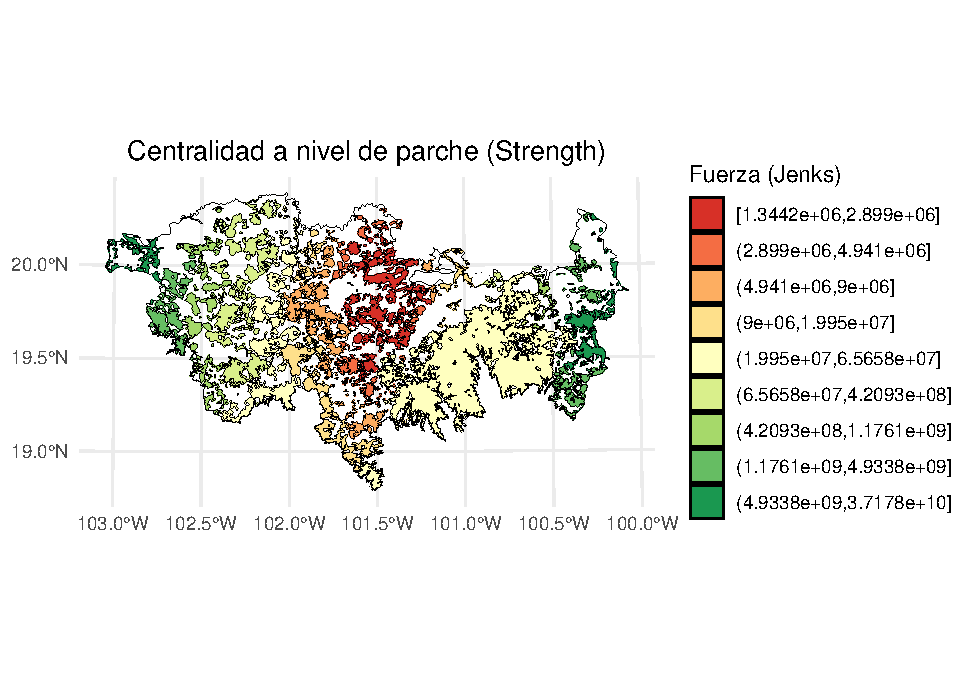
\includegraphics[keepaspectratio]{03-Centralidad_files/figure-latex/unnamed-chunk-7-1.pdf}}

\begin{itemize}
\tightlist
\item
  BWC:
\end{itemize}

\begin{Shaded}
\begin{Highlighting}[]
\NormalTok{breaks }\OtherTok{\textless{}{-}}\NormalTok{ classInt}\SpecialCharTok{::}\FunctionTok{classIntervals}\NormalTok{(centrality\_test}\SpecialCharTok{$}\NormalTok{BWC, }\AttributeTok{n =} \DecValTok{9}\NormalTok{, }\AttributeTok{style =} \StringTok{"jenks"}\NormalTok{)}
\NormalTok{centrality\_test }\OtherTok{\textless{}{-}}\NormalTok{ centrality\_test }\SpecialCharTok{\%\textgreater{}\%}
  \FunctionTok{mutate}\NormalTok{(}\AttributeTok{BWC\_jenks =} \FunctionTok{cut}\NormalTok{(BWC,}
                              \AttributeTok{breaks =}\NormalTok{ breaks}\SpecialCharTok{$}\NormalTok{brks,}
                              \AttributeTok{include.lowest =} \ConstantTok{TRUE}\NormalTok{,}
                              \AttributeTok{dig.lab =} \DecValTok{5}\NormalTok{))}
\FunctionTok{ggplot}\NormalTok{() }\SpecialCharTok{+}  
  \FunctionTok{geom\_sf}\NormalTok{(}\AttributeTok{data =}\NormalTok{ paisaje, }\AttributeTok{fill =} \ConstantTok{NA}\NormalTok{, }\AttributeTok{color =} \StringTok{"black"}\NormalTok{) }\SpecialCharTok{+}
  \FunctionTok{geom\_sf}\NormalTok{(}\AttributeTok{data =}\NormalTok{ centrality\_test, }\FunctionTok{aes}\NormalTok{(}\AttributeTok{fill =}\NormalTok{ BWC\_jenks), }\AttributeTok{color =} \StringTok{"black"}\NormalTok{, }\AttributeTok{size =} \FloatTok{0.1}\NormalTok{) }\SpecialCharTok{+}
  \FunctionTok{scale\_fill\_brewer}\NormalTok{(}\AttributeTok{palette =} \StringTok{"RdYlGn"}\NormalTok{, }\AttributeTok{direction =} \DecValTok{1}\NormalTok{, }\AttributeTok{name =} \StringTok{"BWC (Jenks)"}\NormalTok{) }\SpecialCharTok{+}
  \FunctionTok{theme\_minimal}\NormalTok{() }\SpecialCharTok{+}
  \FunctionTok{labs}\NormalTok{(}
    \AttributeTok{title =} \StringTok{"Centralidad a nivel de parche (BWC)"}\NormalTok{,}
    \AttributeTok{fill =} \StringTok{"BWC}\SpecialCharTok{\textbackslash{}n}\StringTok{(Jenks)"}
\NormalTok{  ) }\SpecialCharTok{+}
  \FunctionTok{theme}\NormalTok{(}
    \AttributeTok{legend.position =} \StringTok{"right"}\NormalTok{,}
    \AttributeTok{plot.title =} \FunctionTok{element\_text}\NormalTok{(}\AttributeTok{hjust =} \FloatTok{0.5}\NormalTok{)}
\NormalTok{  )}
\end{Highlighting}
\end{Shaded}

\pandocbounded{\includegraphics[keepaspectratio]{03-Centralidad_files/figure-latex/unnamed-chunk-8-1.pdf}}

\begin{itemize}
\tightlist
\item
  Membresía por random walk:
\end{itemize}

\begin{Shaded}
\begin{Highlighting}[]
\FunctionTok{ggplot}\NormalTok{() }\SpecialCharTok{+}  
  \FunctionTok{geom\_sf}\NormalTok{(}\AttributeTok{data =}\NormalTok{ paisaje, }\AttributeTok{fill =} \ConstantTok{NA}\NormalTok{, }\AttributeTok{color =} \StringTok{"black"}\NormalTok{) }\SpecialCharTok{+}
  \FunctionTok{geom\_sf}\NormalTok{(}\AttributeTok{data =}\NormalTok{ centrality\_test, }\FunctionTok{aes}\NormalTok{(}\AttributeTok{fill =} \FunctionTok{as.factor}\NormalTok{(memb.rw)), }\AttributeTok{color =} \StringTok{"black"}\NormalTok{, }\AttributeTok{size =} \FloatTok{0.1}\NormalTok{) }\SpecialCharTok{+}
  \FunctionTok{scale\_fill\_brewer}\NormalTok{(}
    \AttributeTok{palette =} \StringTok{"Set3"}\NormalTok{,}
    \AttributeTok{name =} \StringTok{"Membership RW"}
\NormalTok{  ) }\SpecialCharTok{+}
  \FunctionTok{theme\_minimal}\NormalTok{() }\SpecialCharTok{+}
  \FunctionTok{labs}\NormalTok{(}
    \AttributeTok{title =} \StringTok{"Agrupación de parches (Random walks)"}\NormalTok{,}
    \AttributeTok{fill =} \StringTok{"Membership RW"}
\NormalTok{  ) }\SpecialCharTok{+}
  \FunctionTok{theme}\NormalTok{(}
    \AttributeTok{legend.position =} \StringTok{"right"}\NormalTok{,}
    \AttributeTok{plot.title =} \FunctionTok{element\_text}\NormalTok{(}\AttributeTok{hjust =} \FloatTok{0.5}\NormalTok{)}
\NormalTok{  )}
\end{Highlighting}
\end{Shaded}

\pandocbounded{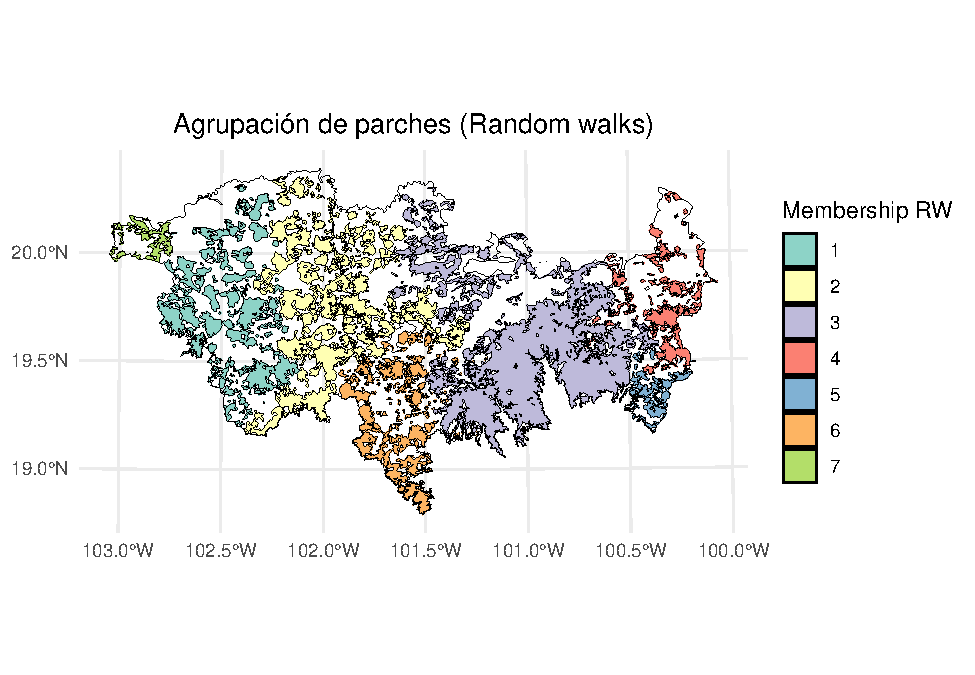
\includegraphics[keepaspectratio]{03-Centralidad_files/figure-latex/unnamed-chunk-9-1.pdf}}

\begin{itemize}
\tightlist
\item
  Membresía por Louvain:
\end{itemize}

\begin{Shaded}
\begin{Highlighting}[]
\FunctionTok{ggplot}\NormalTok{() }\SpecialCharTok{+}  
  \FunctionTok{geom\_sf}\NormalTok{(}\AttributeTok{data =}\NormalTok{ paisaje, }\AttributeTok{fill =} \ConstantTok{NA}\NormalTok{, }\AttributeTok{color =} \StringTok{"black"}\NormalTok{) }\SpecialCharTok{+}
  \FunctionTok{geom\_sf}\NormalTok{(}\AttributeTok{data =}\NormalTok{ centrality\_test, }\FunctionTok{aes}\NormalTok{(}\AttributeTok{fill =} \FunctionTok{as.factor}\NormalTok{(memb.louvain)), }\AttributeTok{color =} \StringTok{"black"}\NormalTok{, }\AttributeTok{size =} \FloatTok{0.1}\NormalTok{) }\SpecialCharTok{+}
  \FunctionTok{scale\_fill\_brewer}\NormalTok{(}
    \AttributeTok{palette =} \StringTok{"Set3"}\NormalTok{,}
    \AttributeTok{name =} \StringTok{"Membership LV"}
\NormalTok{  ) }\SpecialCharTok{+}
  \FunctionTok{theme\_minimal}\NormalTok{() }\SpecialCharTok{+}
  \FunctionTok{labs}\NormalTok{(}
    \AttributeTok{title =} \StringTok{"Agrupación de parches (Louvain)"}\NormalTok{,}
    \AttributeTok{fill =} \StringTok{"Membership LV"}
\NormalTok{  ) }\SpecialCharTok{+}
  \FunctionTok{theme}\NormalTok{(}
    \AttributeTok{legend.position =} \StringTok{"right"}\NormalTok{,}
    \AttributeTok{plot.title =} \FunctionTok{element\_text}\NormalTok{(}\AttributeTok{hjust =} \FloatTok{0.5}\NormalTok{)}
\NormalTok{  )}
\end{Highlighting}
\end{Shaded}

\pandocbounded{\includegraphics[keepaspectratio]{03-Centralidad_files/figure-latex/unnamed-chunk-10-1.pdf}}

\section{Ejemplo 2}\label{ejemplo-2}

Usando más de un umbral de distancia

\begin{Shaded}
\begin{Highlighting}[]
\NormalTok{centrality\_test }\OtherTok{\textless{}{-}} \FunctionTok{MK\_RMCentrality}\NormalTok{(}\AttributeTok{nodes =}\NormalTok{ habitat\_nodes,}
                                \AttributeTok{distance =} \FunctionTok{list}\NormalTok{(}\AttributeTok{type =} \StringTok{"centroid"}\NormalTok{),}
                                 \AttributeTok{distance\_thresholds =} \FunctionTok{c}\NormalTok{(}\DecValTok{10000}\NormalTok{, }\DecValTok{100000}\NormalTok{),}
                                 \AttributeTok{probability =} \FloatTok{0.5}\NormalTok{,}
                                 \AttributeTok{write =} \ConstantTok{NULL}\NormalTok{)}
\CommentTok{\#\textgreater{} Done!}
\NormalTok{centrality\_test}
\CommentTok{\#\textgreater{} $d10000}
\CommentTok{\#\textgreater{} Simple feature collection with 404 features and 8 fields}
\CommentTok{\#\textgreater{} Geometry type: POLYGON}
\CommentTok{\#\textgreater{} Dimension:     XY}
\CommentTok{\#\textgreater{} Bounding box:  xmin: {-}108954 ymin: 2025032 xmax: 202330.2 ymax: 2198936}
\CommentTok{\#\textgreater{} Projected CRS: NAD\_1927\_Albers}
\CommentTok{\#\textgreater{} First 10 features:}
\CommentTok{\#\textgreater{}    Id strength        eigen      close  BWC cluster memb.rw}
\CommentTok{\#\textgreater{} 1   1 30228524 0.0010435836 0.03840356    0       1       6}
\CommentTok{\#\textgreater{} 2   2 21600031 0.0006195356 0.03995935    1       1       6}
\CommentTok{\#\textgreater{} 3   3 29320545 0.0009026418 0.03831019    0       1       6}
\CommentTok{\#\textgreater{} 4   4 16499522 0.0005867564 0.04187906   23       1       6}
\CommentTok{\#\textgreater{} 5   5 26068911 0.0011987437 0.04240465    0       1       6}
\CommentTok{\#\textgreater{} 6   6 12737692 0.0005630043 0.04627714   17       1       6}
\CommentTok{\#\textgreater{} 7   7 12497243 0.0005499038 0.04634291   15       1       6}
\CommentTok{\#\textgreater{} 8   8 13198398 0.0005859873 0.04607765    0       1       6}
\CommentTok{\#\textgreater{} 9   9 22276433 0.0010276194 0.04296412  567       1       6}
\CommentTok{\#\textgreater{} 10 10 12804425 0.0004306005 0.04405417 1063       1       6}
\CommentTok{\#\textgreater{}    memb.louvain                       geometry}
\CommentTok{\#\textgreater{} 1             1 POLYGON ((54911.05 2035815,...}
\CommentTok{\#\textgreater{} 2             2 POLYGON ((44591.28 2042209,...}
\CommentTok{\#\textgreater{} 3             2 POLYGON ((46491.11 2042467,...}
\CommentTok{\#\textgreater{} 4             1 POLYGON ((54944.49 2048163,...}
\CommentTok{\#\textgreater{} 5             1 POLYGON ((80094.28 2064140,...}
\CommentTok{\#\textgreater{} 6             1 POLYGON ((69205.24 2066394,...}
\CommentTok{\#\textgreater{} 7             1 POLYGON ((68554.2 2066632, ...}
\CommentTok{\#\textgreater{} 8             1 POLYGON ((69995.53 2066880,...}
\CommentTok{\#\textgreater{} 9             1 POLYGON ((79368.68 2067324,...}
\CommentTok{\#\textgreater{} 10            2 POLYGON ((23378.32 2067554,...}
\CommentTok{\#\textgreater{} }
\CommentTok{\#\textgreater{} $\textasciigrave{}d1e+05\textasciigrave{}}
\CommentTok{\#\textgreater{} Simple feature collection with 404 features and 8 fields}
\CommentTok{\#\textgreater{} Geometry type: POLYGON}
\CommentTok{\#\textgreater{} Dimension:     XY}
\CommentTok{\#\textgreater{} Bounding box:  xmin: {-}108954 ymin: 2025032 xmax: 202330.2 ymax: 2198936}
\CommentTok{\#\textgreater{} Projected CRS: NAD\_1927\_Albers}
\CommentTok{\#\textgreater{} First 10 features:}
\CommentTok{\#\textgreater{}    Id strength     eigen     close BWC cluster memb.rw}
\CommentTok{\#\textgreater{} 1   1 958.4815 0.6679253 0.4207380   0       1       1}
\CommentTok{\#\textgreater{} 2   2 925.0415 0.6471542 0.4356561   0       1       1}
\CommentTok{\#\textgreater{} 3   3 960.2533 0.6700437 0.4197704   0       1       1}
\CommentTok{\#\textgreater{} 4   4 896.6891 0.6266304 0.4494531   0       1       1}
\CommentTok{\#\textgreater{} 5   5 871.2094 0.6057986 0.4632174   0       1       1}
\CommentTok{\#\textgreater{} 6   6 836.4790 0.5842254 0.4818295   0       1       1}
\CommentTok{\#\textgreater{} 7   7 836.5028 0.5843345 0.4818097   0       1       1}
\CommentTok{\#\textgreater{} 8   8 837.6158 0.5848721 0.4811889   0       1       1}
\CommentTok{\#\textgreater{} 9   9 858.0974 0.5971238 0.4701554   0       1       1}
\CommentTok{\#\textgreater{} 10 10 874.7611 0.6125436 0.4606972   0       1       1}
\CommentTok{\#\textgreater{}    memb.louvain                       geometry}
\CommentTok{\#\textgreater{} 1             1 POLYGON ((54911.05 2035815,...}
\CommentTok{\#\textgreater{} 2             1 POLYGON ((44591.28 2042209,...}
\CommentTok{\#\textgreater{} 3             1 POLYGON ((46491.11 2042467,...}
\CommentTok{\#\textgreater{} 4             1 POLYGON ((54944.49 2048163,...}
\CommentTok{\#\textgreater{} 5             1 POLYGON ((80094.28 2064140,...}
\CommentTok{\#\textgreater{} 6             1 POLYGON ((69205.24 2066394,...}
\CommentTok{\#\textgreater{} 7             1 POLYGON ((68554.2 2066632, ...}
\CommentTok{\#\textgreater{} 8             1 POLYGON ((69995.53 2066880,...}
\CommentTok{\#\textgreater{} 9             1 POLYGON ((79368.68 2067324,...}
\CommentTok{\#\textgreater{} 10            1 POLYGON ((23378.32 2067554,...}
\end{Highlighting}
\end{Shaded}

10 km:

\begin{Shaded}
\begin{Highlighting}[]
\FunctionTok{plot}\NormalTok{(centrality\_test}\SpecialCharTok{$}\NormalTok{d10000[}\StringTok{"BWC"}\NormalTok{], }\AttributeTok{breaks =} \StringTok{"jenks"}\NormalTok{)}
\end{Highlighting}
\end{Shaded}

\pandocbounded{\includegraphics[keepaspectratio]{03-Centralidad_files/figure-latex/unnamed-chunk-12-1.pdf}}

100 km:

\begin{Shaded}
\begin{Highlighting}[]
\FunctionTok{plot}\NormalTok{(centrality\_test}\SpecialCharTok{$}\StringTok{\textasciigrave{}}\AttributeTok{d1e+05}\StringTok{\textasciigrave{}}\NormalTok{[}\StringTok{"BWC"}\NormalTok{], }\AttributeTok{breaks =} \StringTok{"quantile"}\NormalTok{)}
\end{Highlighting}
\end{Shaded}

\pandocbounded{\includegraphics[keepaspectratio]{03-Centralidad_files/figure-latex/unnamed-chunk-13-1.pdf}}

  \bibliography{book.bib,packages.bib}

\end{document}
